\documentclass[11pt,twoside,a4paper]{book}

\usepackage[czech, english]{babel}
\usepackage[OT1]{fontenc} % pouzije EC fonty
\usepackage[utf8]{inputenc}
\usepackage{lmodern}
\usepackage{graphicx}

\usepackage{mathtools}
\usepackage{indentfirst} %1. odstavec jako v cestine.
\usepackage{k336_thesis_macros} 
\usepackage{hyperref}
\hypersetup{
    bookmarks=true,         % show bookmarks bar?
    unicode=true,		% non-Latin characters in Acrobat’s bookmark
    colorlinks=true,       	% false: boxed links; true: colored links
    linkcolor=blue,		% color of internal links (change box color with linkbordercolor)
    citecolor=blue,        	% color of links to bibliography
}

\usepackage[square, numbers]{natbib}             % sazba pouzite literatury

\usepackage{listings}
\usepackage{courier}
\lstset{
	language=C++,
	frame=single,
	basicstyle=\footnotesize\ttfamily,
	commentstyle=\color{gray},
	keywordstyle=\color{blue},
	stringstyle=\color{BurntOrange},
	numbers=left,
	captionpos=b,
	numberstyle=\tiny\ttfamily,
	%stepnumber=2,
	numbersep=5pt,
	tabsize=2,
	showstringspaces=false,
	extendedchars=true,
	breaklines=true,
	frame=tb,
	xleftmargin=17pt,
	framexleftmargin=17pt,
	framexrightmargin=5pt,
	framexbottommargin=4pt,
}
\renewcommand*\lstlistingname{Zdrojový kód}
\usepackage{color}
\usepackage[usenames,dvipsnames]{xcolor}

\usepackage{textcomp}


\newcommand\Department{Katedra počítačů}
\newcommand\Faculty{Fakulta elektrotechnická}
\newcommand\University{České vysoké učení technické v Praze}
\newcommand\labelSupervisor{Vedoucí práce}
\newcommand\labelStudProgram{Studijní program}
\newcommand\labelStudBranch{Obor}

\newcommand\TypeOfWork{Diplomová práce} \typeout{Diplomova prace}
\newcommand\StudProgram{Otevřená informatika, Magisterský}
\newcommand\StudBranch{Softwarové inženýrství}

\newcommand\WorkTitle{Pohledově závislá aplikace textur v reálném čase}
\newcommand\FirstandFamilyName{Bc. Daniel Princ} \newcommand\Supervisor{Ing.
David Sedláček, Ph.D.}


\let\oldUrl\url \renewcommand\url[1]{<\texttt{\oldUrl{#1}}>}

\begin{document}
\selectlanguage{czech} 

\coverpagestarts

\acknowledgements \noindent \noindent Chtěl bych poděkovat vedoucímu této práce,
panu Ing. Davidovi Sedláčkovi, Ph.D., za poskytnutí cenných rad a nápadů.

\declaration{V~Praze,  12. 5. 2014}
 
\abstractpage
TBD

\vglue60mm

\tableofcontents

\listoffigures

\listoftables

\renewcommand*{\lstlistlistingname}{Seznam zdrojových kódů}
\lstlistoflistings

\mainbodystarts
% horizontalní mezera mezi dvema odstavci \parskip=5pt 11.12.2008 parskip +
% tolerance
\normalfont \parskip=0.2\baselineskip plus 0.2\baselineskip minus
0.1\baselineskip


\chapter{Úvod}
V dnešní době umožňuje počítačová grafika renderovat realistické obrazy 3D
světa. Nicméně aby toto bylo možné, musí existovat 3D modely objektů, které
chceme zobrazovat. Tradiční způsob, jak získat tyto modely, je jejich ruční
vytváření v modelovacích programech. To je velmi pracný a zdlouhavý proces
a~jeho výsledek není dostatečně realistický. Proto se v současnosti vyvíjí
postupy, jak přímo digitalizovat reálné objekty. Existují dva základní přístupy,
které se o toto pokoušejí. Nejpřesnější metoda je pravděpodobně laserové
skenování objektů. Druhou, mnohem levnější a dostupnější variantou, je rekonstrukce objektů z
fotografií. Těmito problémy se zabývá počítačové vidění a částečně také
počítačová grafika, do které spadá zobrazování rekonstruovaných modelů. Cílem 3D
počítačové rekonstrukce je tedy co nejvěrněji převést reálné objekty do
digitální podoby. Aplikaci najdeme ve virtuální realitě, online prohlídkách,
počítačových animacích nebo v herním či filmovém průmyslu.

Tato práce se zabývá jednou částí 3D rekonstrukce a to texturování objektů z
fotografií. Na vstupu očekáváme již zrekonstruovaný 3D model (síť trojúhelníků)
a větší množství (desítky až stovky) kalibrovaných fotografií z různých úhlů. Textura společně s materiálem slouží k popisu povrchu a je důležitá pro vnímání barvy a detailní struktury povrchu \cite{mpg}. Aplikace textury vede z výraznému zvýšení vizuální kvality objektu za relativně malou cenu.  Často je vizuálně i výkonově jednodušší použít detailní texturu a jednoduchý model s menším počtem vrcholů, viz obr. \ref{fig:example}.

\begin{figure}[h]
\begin{center}
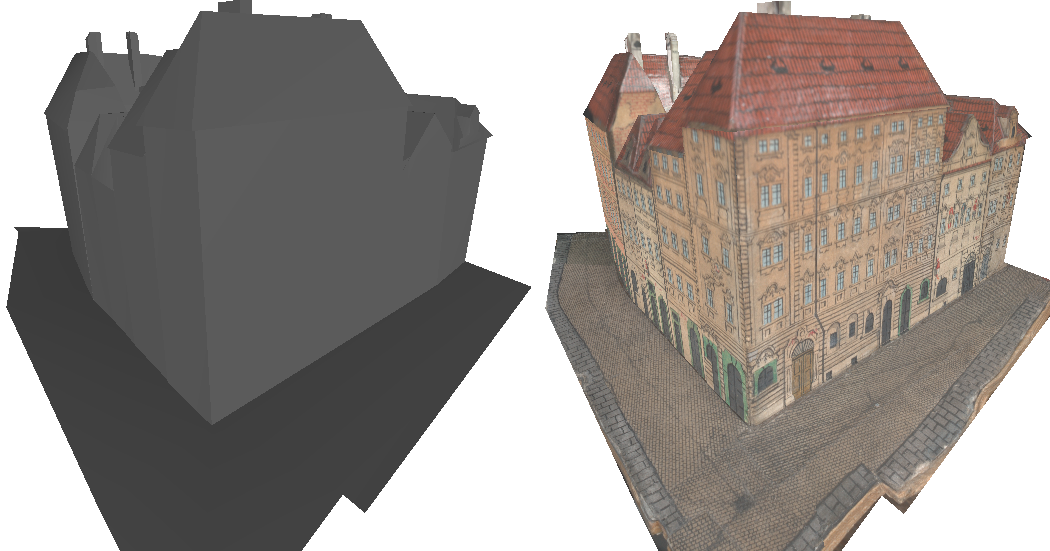
\includegraphics[width=\textwidth]{figures/example}
\caption{Ukázka 3D modelu bez textur (vlevo) a s texturami (vpravo).}
\label{fig:example}
\end{center}
\end{figure}

Syntéza textur z fotografií je poměrně složitá, protože 	na výsledný model se díváme i z jiných pohledů, než ze kterých byly pořízeny fotografie. Problémy, které při tomto procesu vznikají jsou popsány zejména v následující kapitole. Cílem této práce je vytvořit aplikaci, která v reálném čase mapuje fotografie na model. Protože aplikace funguje v reálném čase, může zohlednit aktuální pohled virtuální kamery a na základě pozice kamery vybrat nejvhodnější fotografie pro vytvoření textury. K tomu využívá velkého výkonu současných GPU.

\newpage
\section{Struktura práce}

Práce v kapitole \ref{chap:analysis} rozebírá zadaný problém a popisuje související práce. Poté se věnuje popisu navrhované metody a řešení problémů. Kapitola \ref{chap:impl} popisuje implementaci naší metody. Poté je v kapitole \ref{chap:testing} provedeno testování aplikace na různých scénách. V závěru v kapitole \ref{chap:end} jsou diskutovány výsledky testování a jsou navrženy možné vylepšení metody a implementace.

\chapter{Analýza problému a návrh řešení}
\label{chap:analysis}
\section{Popis problému}

Předpokládejme, že se díváme na statickou scénu s konstantním osvětlením, kde se pohybuje pouze pozorovatel. Za těchto podmínek můžeme popsat libovolnou fotografii pomocí pozice a orientace kamery. Pokud bychom vyfotili sférickou fotografii v každé možné pozici kamery, mohli bychom vyrenderovat kompletní scénu z libovolného pohledu. Kombinací všech 3D pozic kamery $(x, y, z)$ a směrů $(\theta, \phi)$ získáme plenoptickou funkci $\textbf{L}(x, y, z, \theta, \phi)$ \cite{Adelson91}. Snahou je aproximovat funkci \textbf{L} pomocí konečného množství diskrétních vzorků $(x, y, z, \theta, \phi)$ a z této reprezentace efektivně renderovat nové pohledy (s pomocí 3D geometrie) \cite{floating-textures}. Povrch geometrie můžeme popsat jako funkci $\textbf{G} : (x, y, z, \theta, \phi) \to (x_0, y_0, z_0)$, tedy jako mapování pohledových paprsků na 3D souřadnice povrchu. Jako $\textbf{G}_0$ si označíme funkci skutečného povrchu, $\textbf{G}_A$  reprezentuje aproximovaný povrch (rekonstruovaný 3D model), viz obr. \ref{fig:projection-error}.

\begin{figure}[hb]
\begin{center}
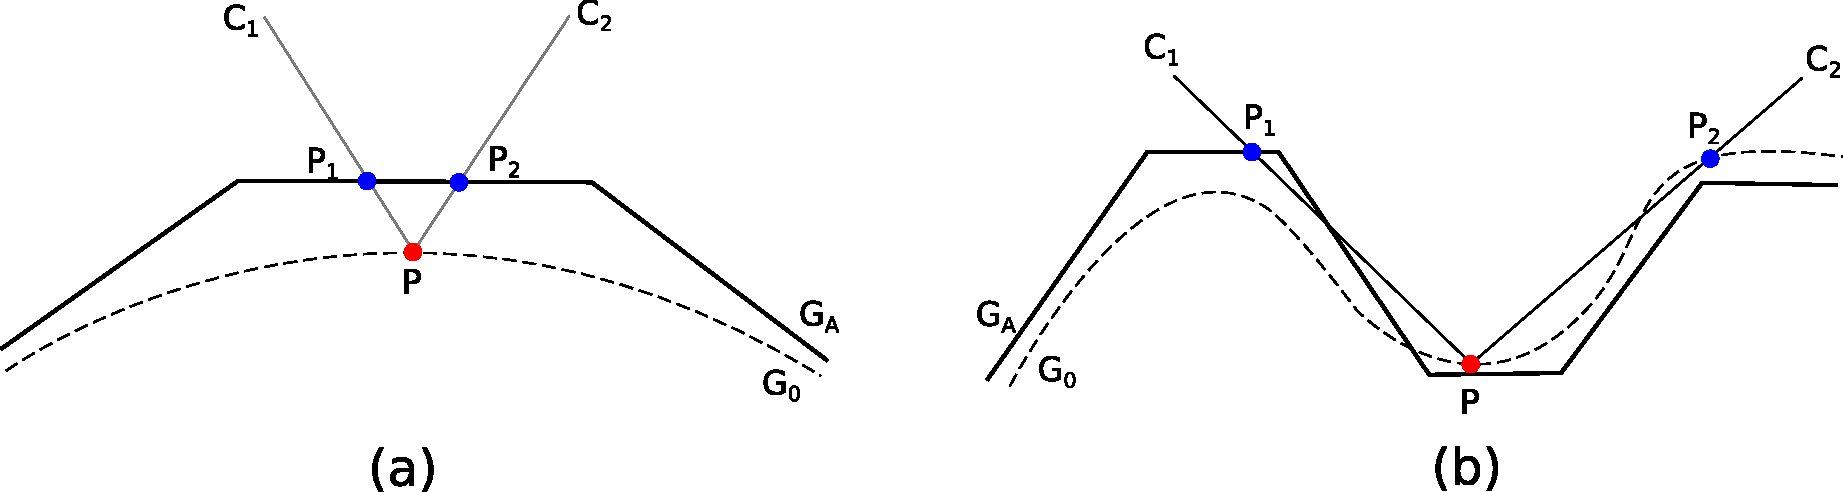
\includegraphics[width=\textwidth]{figures/projection-error}
\caption{(a) Chyby v geometrii způsobují chybnou projekci, bod P na původní geometrii je promítnut na body $P_1$ a $P_2$ na aproximované geometrii. (b) Chyby ve viditelnosti, bod P je chybně viditelný z kamery $C_2$ a naopak není viditelný z kamery $C_1$.}
\label{fig:projection-error}
\end{center}
\end{figure}

Důležitým prvkem je projekční matice kamery, která nám určuje projekční mapování 3D bodu $(x, y, z)$ do 2D souřadnic $(s, t)$ v $i$-té fotografii  $\textbf{P}_i: (x, y, z) \to (s, t)$, viz sekce \ref{sec:matice-kamery}.  Z promítnuté pozice v obrázku pak můžeme přiřadit 3D bodu barvu $\textbf{I}_i : (s, t) \to (r, g, b)$. Poté libovolný nový pohled $\textbf{I}^V$ z virtuální kamery $V$ můžeme vyjádřit pomocí rovnice \ref{eq:iview}.

\begin{align}
\label{eq:iview}
\textbf{I}^V(x, y, z, \theta, \phi) = \sum_{i} \textbf{I}_{i}^{V}(x, y, z, \theta, \phi)~\omega_i
\end{align}

\noindent kde

\begin{align}
\label{eq:linear-comb-plen}
\textbf{I}_{i}^{V}(x, y, z, \theta, \phi) &=\textbf{I}_{i}(\textbf{P}_{i}(\textbf{G}_A(x, y, z, \theta, \phi)))\\
\label{eq:linear-weighting}
 \omega_i &= \delta_i(\textbf{G}_A(x, y, z, \theta, \phi)) w_i(x, y, z, \theta, \phi)
\end{align}

\noindent a $\sum_i \omega_i = 1$. Notace $ \textbf{I}_{i}^{V}$ značí vyrenderovaný obrázek z pohledu $V$ promítnutím vstupní fotografie  $\textbf{I}_{i}$ jako textury na povrch  $\textbf{G}_A$. $\delta_i$ určuje viditelnost a je 1, pokud je bod na povrchu $\textbf{G}_A$ viditelný v kameře $i$ a 0 pokud není. $w_i$ je funkce, která určuje váhu kamery $i$ pro každý paprsek. Rovnice \ref{eq:iview} se snaží reprezentovat plenoptickou funkci jako lineární kombinaci promítnutých fotografií.

Zásadní problém spočívá v tom, že $\textbf{G}_A \neq \textbf{G}_0$, tedy již vstupní data vztahu \ref{eq:linear-comb-plen} jsou zatížena chybou (obr. \ref{fig:projection-error}). Problémy přináší také nepřesná kalibrace kamery $\textbf{P}_i$, což způsobuje další nepřesnosti při mapování.

\section{Související práce}
\label{sec:related}

Existuje několik základních metod, jak mapovat fotografie z více pohledů na
model, většina metod ale funguje na stejném principu:
\begin{enumerate}
\item Extrakce textur z fotografií pomocí vrhání paprsků či jiné podobné metody.
\item Vzájemná registrace textur
\item Sloučení textur do výsledné textury 
\end{enumerate}

Jednou z možností je projekce všech fotografií a jejich následné sloučení
pomocí nějakého váženého průměru, jako např. v \cite{Bernardini01}.
Nevýhodou takové metody je zejména vznik artefaktů ve výsledné textuře, často se
projevuje tzv. ghosting, kdy se v textuře objeví několik kopií jednoho obrazce.
Další variantou je vytvoření atlasu textur \cite{Allene08}, kdy každá část
modelu dostane svojí texturu z unikátního pohledu. Tato varianta je využita
např. v \cite{multi-view-tex}. Tento přístup má nevýhodu ve vzniku švů na
okrajích jednotlivých částí textur, které je pak nutné odstraňovat
\cite{seamless-mosaicing}. Kromě artefaktů je u těchto přístupů častým problémem
rozostření některých částí textur. Většina zmiňovaných problémů vzniká kvůli
nepřesné kalibraci fotografií (špatnému odhadu radiální distorze či ohniskové
vzdálenosti) nebo nepřesně rekonstruovaným modelům. Tyto nepřesnosti jsou
obvyklé, i když jsou dnes již algoritmy pro 3D rekonstrukci velmi kvalitní.
Získat velmi přesně kalibrované fotografie je časově náročný proces a někdy i
téměř nerealizovatelný, např. ve venkovních scénách.

V článku \cite{multi-view-tex} jsou uvažovány nepřesně vytvořené modely, které
je nutné otexturovat z původních fotografií, i když na model přesně nepasují.
Navrhují podle modelu upravit původní fotografie a z nich následně vytvořit
atlas textur. Úpravu provádí tak, že ve fotografiích identifikují významné
prvky, které naleznou na vytvořeném modelu a zpětně je promítají do původních
pohledů. Poté deformují všechny fotografie, aby co nejlépe odpovídaly nepřesným
modelům. Touto metodou se nezbaví všech artefaktů, ale omezí jejich výskyt.

Podobný přístup je použitý v \cite{harmonized-texture-mapping}, kde je
popsán způsob, jak dynamicky deformovat několik textur najednou podle 3D modelu
a poté je pomocí vážených faktorů sloučit dohromady na základě pozice virtuální
kamery.

Odlišný přístup je použitý v článku \cite{masked-blending}. Zde řeší texturování
hustých modelů s jednotkami až desítkami milionů trojúhelníků. Pro takto husté
modely nepoužívají textury, ale barvu přiřazují pouze vrcholům, což vzhledem k
počtu vrcholů v modelu poskytuje dostatečné detaily. Základní princip algoritmu
je takový, že model je vykreslen z pohledu jednotlivých kamer a poté jsou
viditelné vrcholy promítnuty zpět do původních fotografií. Pokud je jeden vrchol
vidět na více fotografiích, je použita funkce, která vybere nejvhodnější barvu
pro daný vrchol. Tato funkce používá vážené masky, které jsou vygenerovány pro
každou fotografii a udávají kvalitu jednotlivých pixelů. Pro určení kvality
pixelu je použito několik různých metrik, pro každou fotografii je tedy
vytvořeno více masek (každá maska má rozlišení stejné jako fotografie). Použité
metriky jsou následující:
\begin{itemize}
  \item Úhlová metrika - nejjednodušší metrika, která porovnává směr ke kameře s 
  		normálou plochy. Největší váha je, pokud jsou oba směry stejné.
  \item Hloubková metrika - váha pixelu je větší, pokud je povrch blíže ke 
  		kameře.
  \item Hraniční metrika - tato maska udává, jak daleko je pixel od okrajů 
  		fotografie a siluety v hloubkové mapě. Čím dále je pixel od okrajů, 
  		tím je jeho kvalita lepší.
\end{itemize}
Výsledná váha pixelu je získána vynásobením hodnot v jednotlivých maskách. Tím 
je zaručeno zachování lokálních minim v každé masce, což pomáhá odstraňovat 
pixely, které jsou v libovolné masce považovány za velmi špatné. Výsledná barva 
pro každý vrchol se získá porovnáním masek u všech fotografií, ze kterých je daný 
vrchol viditelný, a následným vybráním nejlepšího pixelu.

Výhoda tohoto způsobu je, že se nejedná o výpočetně složité operace, většina
výpočtů je prováděna nad fotografiemi a není závislá na složitosti modelu. Další
výhodou je možnost určit kvalitu jednotlivých fotografií podle maximální či
průměrné kvality masky. Tím je možné některé nevhodné fotografie automaticky
eliminovat a zrychlit celý proces. Nevýhodou této metody je nutnost hustých
modelů, u modelů s nižším počtem vrcholů by výsledky této metody nebyly příliš
kvalitní. Další problém nastává, pokud je rozlišení fotografií vyšší než
rozlišení modelu (jeden vrchol se mapuje na více pixelů ve fotografiích), to
vyžaduje další zpracování dat a zvyšuje složitost problému.


Všechny tyto algoritmy mají společné to, že z původních pohledů předem vytvoří
texturu či atlas textur spojením všech fotografií, přičemž se snaží
minimalizovat vznik artefaktů nebo případně vzniklé artefakty odstraňovat.
Metoda navržená v této práci se zásadně liší tím, že žádnou takovou texturu
nevytváří, ale pro každý aktuální pohled virtuální kamery vybírá množinu
fotografií z nejvhodnějších pohledů a z této množiny vybírá nejvhodnější texely.
Zásadní nevýhodou tohoto přístupu je velký výpočetní výkon, který je potřeba při
zobrazování modelu. Tuto nevýhodu se snažíme minimalizovat efektivním využitím
GPU.

Tato myšlenka není úplně nová, na podobném principu je založena např. metoda
plovoucích textur \cite{floating-textures}. Tento algoritmus používá adaptivní
nelineární metodu, která opravuje lokální nezarovnání textur vůči 3D modelu. K
tomu určuje optický tok \footnote{v orig. optical flow} mezi promítanými fotografiemi a
příslušné textury kombinuje.

Navrhovaný postup využívá kombinaci lineární interpolace a odhadu optického
toku. Nejprve je provedena projekce fotografií $I_i$ na model z původních
pohledů a scéna je vyrenderována z aktuálního pohledu virtuální kamery $V$. Tím
vzniknou dočasné textury $I_i^V$. Poté je na jednotlivé páry textur $I_i^V$
aplikován odhad optického toku, čímž vzniknou pole $W_{I_i^V \rightarrow
I_j^V}$. Pro více než dvě vstupní fotografie je nutné provést lineární kombinaci
vytvořených polí a sloučit je do výsledné textury $I^v_{Float}$. To je poměrně náročná operace, pro n vstupních fotografií je nutné vytvořit $O(n^2)$ polí. S tím se vyrovnávají v článku tím, že používají pro každý pohled jen 3 nejbližší fotografie. Plovoucí textury porušují epipolární geometrii, což umožňuje texturám kompenzovat nekvalitní kalibraci kamery a nepřesně zrekonstruované 3D modely.

Dále je nutné vypořádat se s vlastním zastíněním částí modelu, což je velmi
běžná situace. K tomu je využita jemná mapa viditelnosti, která pro každý pixel
určuje, zda je z dané kamery viditelný nebo ne. Oproti tradičním postupům, které
obvykle využívají pouze hodnoty 1 a 0 (je nebo není vidět), je zde použita
metoda, která nastavuje hodnotu z intervalu $(0,1)$ pixelům, které jsou blízko
hranic zastínění. Tím jsou odstraněny ostré hrany podél zastíněných částí, které
jsou velmi často nepřesné a snižují výslednou vizuální kvalitu.

Na principu výběru nejlepší fotografie na základě aktuálního pohledu je založená metoda v článku \cite{Debevec96}. Při mapování jedné fotografie navrhují použití image-space stínových map pro řešení viditelnosti, protože to umožňuje efektivní implementaci pomocí z-bufferu. Při mapování více fotografií na model vybírají pro každý pixel vždy takovou fotografii, která se na daný povrch dívá pod nejlepším úhlem. To samozřejmě přináší viditelné švy, protože sousední pixely mohou pocházet z různých fotografií. Toto řeší zjemněním přechodů pomocí váženého průměru, váhu je určena podle rozdílu úhlu aktuálního pohledu a pohledu původní kamery. Dále pro lepší výsledky mají pixely na okraji fotografie menší váhu, čímž se snaží ještě více eliminovat vznik švů.

Dále navrhují jednoduchý algoritmus pro odstranění nežádoucích objektů, které se mohou vyskytovat na zdrojových fotografiích - např. auto či chodci před budovou, kterou chceme otexturovat. Uživatel může ručně vymaskovat tyto objekty předem zvolenou barvou a tyto pixely dostanou při texturování nulovou váhu a budou použita data z jiné fotografie. Pokud nejsou dostupná žádná data, vyplňují vzniklé mezery pomocí syntézy obrazu.

\section{Návrh řešení}

\subsection{Princip navrhované metody}

Jak již bylo zmíněno v předchozí sekci, tradiční řešení tohoto problému spočívá ve vytvoření jediné textury pomocí sloučení všech vstupních fotografií dohromady. Tento proces je často velmi náročný a zdlouhavý, na stejných testovacích datech, která jsou použita v této práci, trvá proces extrakce textur řádově hodiny \cite{Kirschner08}. Oproti tomu naše navrhované metoda funguje v reálném čase, kdy provádí projekci vybraných fotografií na model. Načtení scény a předzpracování dat pro naší metodu trvá maximálně několik minut. Druhou výhodou našeho řešení je zahrnutí aktuálního pohledu virtuální kamery, které ostatní metody z principu uvažovat nemůžou. Tím se omezí vznik velkého počtu artefaktů v texturách a to jak vznik švů, tak vznik chyb způsobených vlastním zastíněním. Tyto problémy však kompletně nezmizí a je nutné s nimi počítat. 

\begin{figure}[t]
\begin{center}
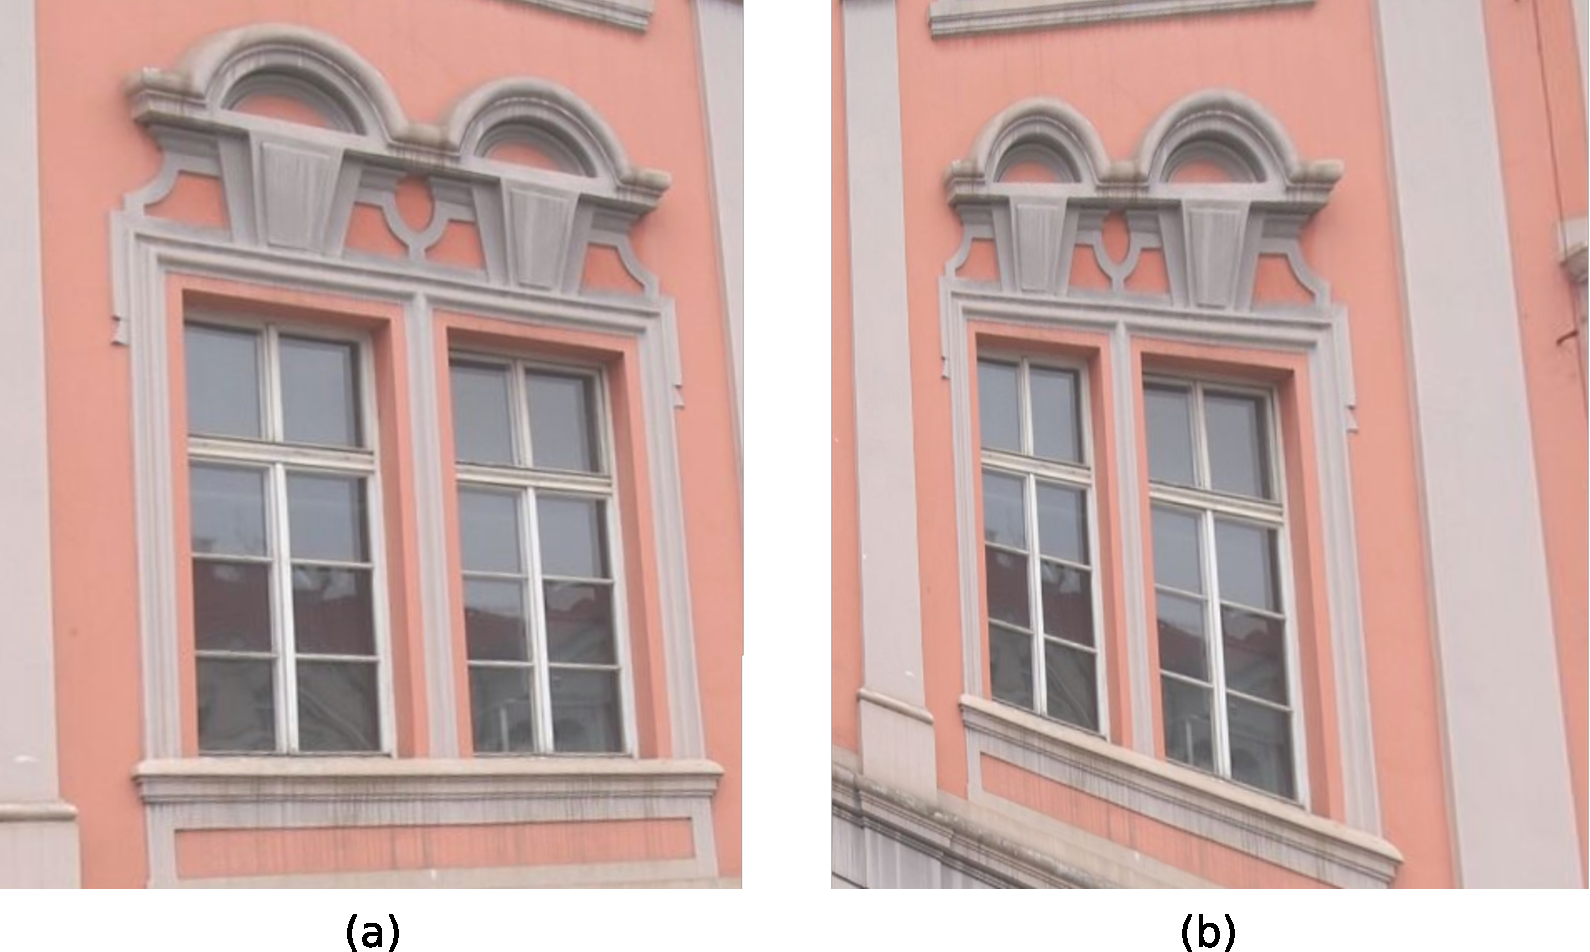
\includegraphics[width=\textwidth]{figures/faust}
\caption{(a) Fotografie namapovaná na model vyrenderovaná z podobného pohledu jako původní fotografie. (b) Stejná fotografie vyrendrovaná z jiného pohledu.}
\label{fig:faust}
\end{center}
\end{figure}

Na obrázku \ref{fig:faust} je zobrazeno namapování fotografie na model bez výrazných geometrických detailů. Pokud je fotografie namapována z podobného úhlu jako je vyfocena původní fotografie, textura působí přirozeně. I když model neobsahuje geometrii okna ani dekorace nad oknem, namapovaná textura vyvolává dojem detailnější 3D geometrie. Oproti tomu stejná textura vyrenderovaná z jiného směru, který je výrazně odlišný od původní fotografie, působí nerealistickým dojmem.


Algoritmus se skládá ze tří základních kroků - projekce fotografií na model, výběr nejlepších fotografií pro pokrytí celého modelu a výběr nejvhodnějšího pixelu z více fotografií pro otexturování fragmentu\footnote{Fragmentem je v textu vždy myšlena plocha na 3D modelu, který odpovídá jednomu výslednému pixelu na obrazovce. Stejně, jako je termín fragment používán v OpenGL.}.

\subsection{Projekce fotografie na model}
\label{sec:matice-kamery}

Mapování jedné fotografie na model můžeme popsat jako projekci $P: (x, y, z) \to (s, t)$, tedy jako projekci 3D bodů modelu do 2D souřadnice ve fotografii, viz obr. \ref{fig:camera-projection}. Nejběžněji se v počítačové grafice a vidění používá perspektivní projekce, která promítá 3D body $p$ na 2D body $x$ vydělením jejich $z$ souřadnicí \cite{Szeliski}. V homogeních souřadnicích má kanonická perspektivní matice \textbf{P}$_0$ jednoduchou formu:
\begin{align}
\label{eq:persp-projection}
x = 
\underbrace{
\begin{bmatrix}
1 & 0 & 0 & 0 \\
0 & 1 & 0 & 0 \\
0 & 0 & 1 & 0 \\
\end{bmatrix}}_\text{\textbf{P}$_0$}
p
\end{align}
\noindent

\begin{figure}[t]
\begin{center}
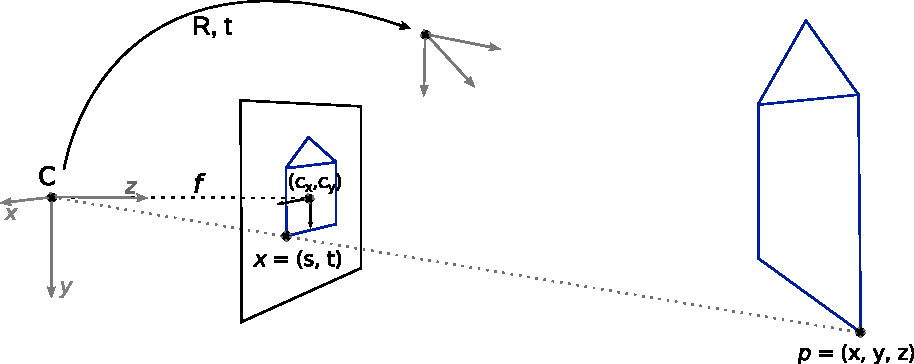
\includegraphics[width=\textwidth]{figures/camera-projection}
\caption{Obrázek znázorňuje situaci při projekci 3D bodu na 2D souřadnice.}
\label{fig:camera-projection}
\end{center}
\end{figure}

Po promítnutí 3D bodu projekční kamerou je nutné transformovat souřadnice na základě vlastností senzoru a orientace kamery vzhledem k počátku souřadnicového systému.  \emph{Kalibrační matice} \textbf{K} transformuje kanonickou perspektivní kameru na standardní projekční kameru \textbf{P}: 
\begin{align}
\label{eq:calibration-matrix}
\textbf{P} = 
\begin{bmatrix}
f & 0 & c_x  \\
0 & f & c_y  \\
0 & 0 & 1  \\
\end{bmatrix}
\cdot
\begin{bmatrix}
1 & 0 & 0 & 0 \\
0 & 1 & 0 & 0 \\
0 & 0 & 1 & 0 \\
\end{bmatrix}
 =\textbf{K}\textbf{P}_0
\end{align}
\noindent
kde $f$ je ohnisková vzdálenost v pixelech a bod $(c_x, c_y)$ je optický střed vyjádřený v pixelech, obr. \ref{fig:camera-projection}. Toto je zjednodušená matice kamery \textbf{K}, která uvažuje senzor kolmý vůči optické ose a stejnou ohniskovou vzdálenost v osách $x$ a $y$ (což je v praxi nejběžnější varianta). Orientaci kamery vůči počátku souřadnicového systému definujeme pomocí $3\times3$ rotační kamery \textbf{R} a vektoru \textbf{t}, čímž získáme výslednou $3\times4$ \emph{matici kamery}:
\begin{align} 
\textbf{P} = \textbf{K}~[~\textbf{R}~|~\textbf{t}~]
\end{align}
\noindent
která provádí mapování bodu $p_w$ v 3D světových souřadnicích do 2D souřadnic $x$ ve fotografii:
\begin{align}
x = \textbf{P}\cdotp p_w
\end{align}
Existuje celá řada algoritmů pro nalezení matice kamery \cite{Hartley2004}, to ale není součástí této práce, kalibrované kamery jsou poskytnuté na vstupu společně s rekonstruovaným modelem a fotografiemi.

Při mapování fotografie na model je nutné brát v úvahu, že některé části modelu mohou být vzhledem ke kameře zastíněné a nemohou být z dané kamery správně otexturovány. Toto se nejčastěji řeší pomocí stínových map \cite{Stamminger2002}, které se předem vytvoří pro každou kameru. Aby byla tato metoda kvalitní, musí mít stínové mapy dostatečné rozlišení.  Vzhledem k tomu, že aplikace bude využívat až stovky různých kamer, bylo by použití této metody paměťově velmi náročné.

Další možností je použít algoritmus vrhání paprsků, kdy se z kamery vrhají na scénu paprsky a podle zásahů s modelem se určí, které fragmenty jsou z kamery viditelné. Tato metoda také není příliš vhodná, protože aplikace bude v reálném čase využívat až desítky různých kamer zároveň a vrhání dostatečného množství paprsků z každé kamery by bylo výpočetně příliš náročné. Proto se jako nejlepší varianta se jeví využít jednodušší algoritmus, který spoléhá na seřazení kamer podle podobnosti se směrem virtuální kamery. Kvůli velkému množství vstupních kamer se dá očekávat, že pro většinu možných pohledů virtuální kamery bude existovat kamera s velmi podobným pohledem. Pro takovou kameru bude existovat jen velmi malé množství oblastí, které budou z kamery zastíněné, ale z virtuální kamery budou viditelné. Při texturování se kamery seřadí od ``nejlepší'' a každá kamera bude využita k otexturování oblasti, která ještě není pokrytá předchozí kamerou. Tím se výrazně omezí oblasti, které jsou otexturovány zastíněnou kamerou, ale zároveň jsou viditelné z virtuální kamery. K tomuto pravidlu je navíc zaveden práh, který určuje minimální úhel mezi směrem kamery a normálou plochy, pro který může být daná plocha kamerou otexturována. 

\newpage
\subsection{Výběr vhodných fotografií pro otexturování modelu}
\label{sec:photo-choosing}

Téměř vždy nestačí k otexturování aktuálního pohledu pouze jedna fotografie. Proto je potřeba použít více fotografií pro vyrenderování modelu z nového pohledu. Na obrázku \ref{fig:dum-1} je zobrazen model s jednou a se dvěma namapovanými fotografiemi.  Při mapování více fotografií zároveň je nutné vyřešit dva základní problémy - které fotografie budou vybrány a jak bude fragment otexturován, pokud je jeho polohu možné promítnout do více kamer.

\begin{figure}[h]
\begin{center}
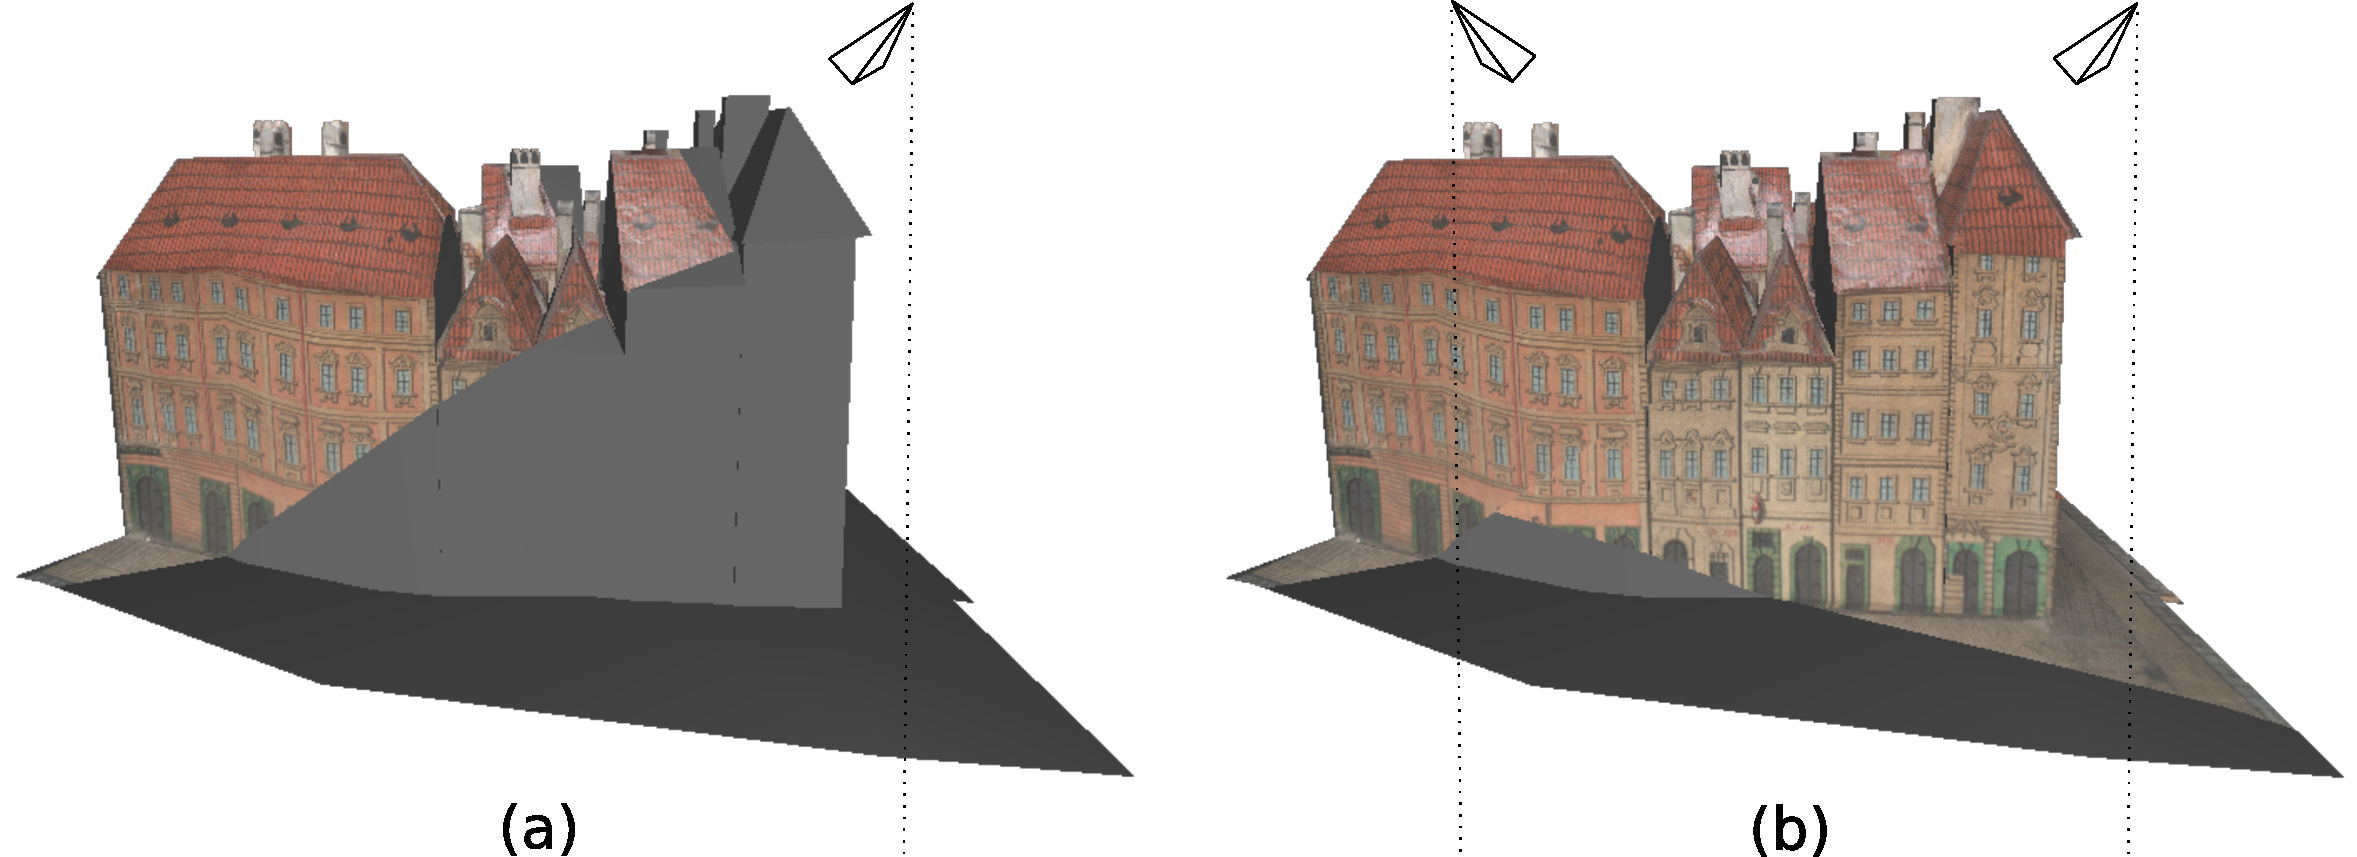
\includegraphics[width=\textwidth]{figures/dum-1}
\caption{Projekce jedné (a) a dvou (b) fotografií na 3D model. Pozice kamer jsou pouze ilustrační.}
\label{fig:dum-1}
\end{center}
\end{figure}

Výběr fotografií je je prováděn na základě shody aktuálního pohledu virtuální kamery s pohledy vstupních kamer. Pro porovnání je nutné určit, kterým směrem jsou kamery natočeny.  U vstupních kamer jde tento směr zjistit přímo z matice kamery, ale nemusí to být vždy výhodné. Pokud se kamera nedívá přímo na objekt (optická osa neprochází objektem), může být směr kamery poměrně zavádějící. Proto navrhujeme algoritmus, který tento směr koriguje na základě viditelné části modelu na fotografii. Tato metoda funguje tak, že se vrcholy rekonstruovaného modelu promítnou do fotografie, body ležící mimo fotografii se zahodí. Poté je nalezena konvexní obálka \cite{Andrew79} promítnutých bodů, která přibližně ohraničuje oblast modelu zobrazenou na fotografii, viz obr. \ref{fig:convex-hull}. Z bodů ležících na konvexní obálce se spočítá centroid a nalezne se směrový vektor ze středu kamery procházející centroidem. Nalezený vektor se použije jako výsledný směr pohledu kamery. Algoritmus není příliš náročný, promítnutí $n$ vrcholů do obrázku je provedeno se složitostí $\Theta(n)$, konvexní obálku ve 2D lze nalézt se složitostí $0(n~log(n))$. Během tohoto algoritmu je zároveň vypočtena plocha konvexní obálky (plocha konvexního polygonu s vrcholy v bodech konvexní obálky). Tato plocha je později při texturování fragmentů zahrnuta do výpočtu váhy fotografie, viz sekce \ref{sec:fragment-texturing}.

\begin{figure}[h]
\begin{center}
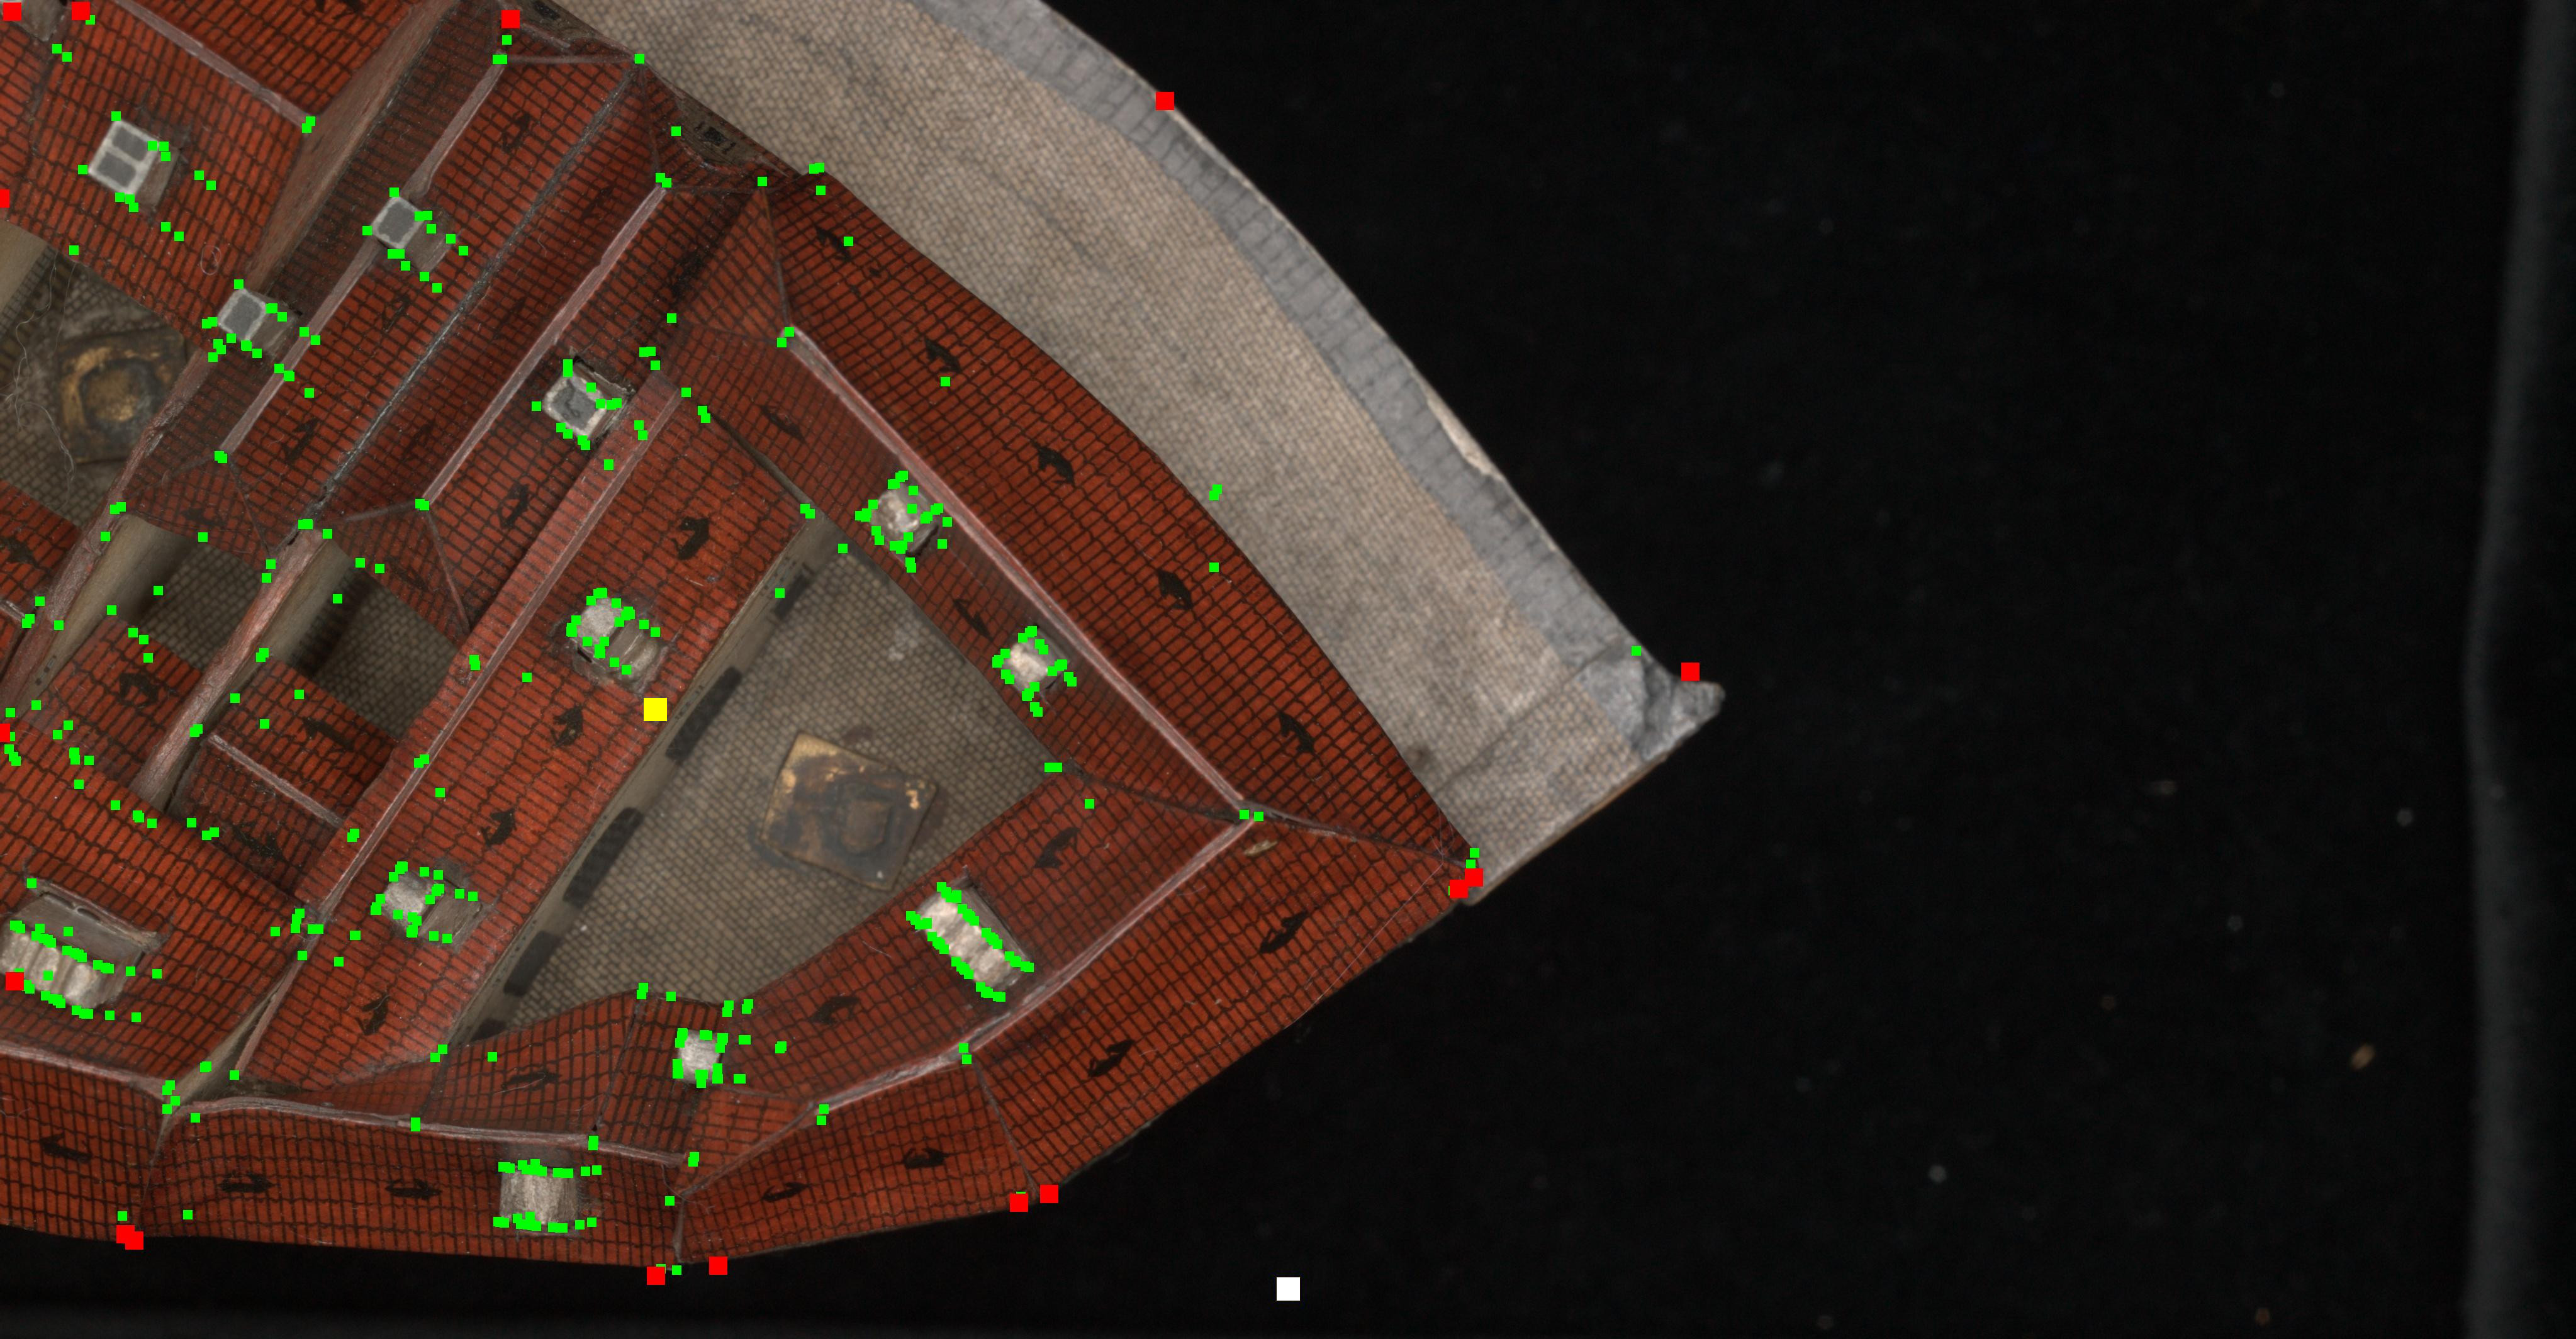
\includegraphics[width=\textwidth]{figures/0-0270_1020_110_09_00_000_098345e}
\caption{Výřez horní poloviny fotografie použité k texturování. Bílý bod označuje průnik optické osy s obrázkem, žlutý bod označuje vypočtený centroid. Ostatní body jsou vrcholy 3D modelu promítnuté do obrázku, červeně zvýrazněné vrcholy leží na konvexní obálce.}
\label{fig:convex-hull}
\end{center}
\end{figure}
 
Podobná situace nastává při určování směru virtuální kamery.  Pokud se díváme zvenku na model a otáčíme virtuální kamerou, vidíme model stále ze stejného směru a chceme, aby byl otexturován stejně. Proto není vhodné použít přímo směr, kterým se dívá virtuální kamera, ale spíše spojnici mezi pozicí kamery a modelem. Pro určení pozice modelu je použit centroid všech vrcholů. Odlišná situace nastává, pokud se virtuální kamera nachází uvnitř modelu. V tomto případě naopak musíme brát v úvahu přímo směr pohledu virtuální kamery, protože při otočení kamery vidíme jinou část modelu. K jednoduchému určení, zda je kamera uvnitř nebo vně modelu, je možné použít osově zarovnaný ohraničující kvádr (AABB).


Po vypočtení směru pohledu vybereme nejlepší fotografie porovnáním se směry všech vstupních kamer. Počet fotografií potřebných k otexturování je závislý na složitosti scény a i na samotných fotografiích, proto se tato hodnota nenastavuje automaticky, ale uživatel jí musí zadat na vstupu.

Pro otexturování modelu často nestačí vybrat pouze fotografie, které nejlépe odpovídají aktuálnímu pohledu. Takové fotografie dobře pokryjí plochy, které jsou na aktuální pohled přibližně kolmé. Oproti tomu velmi špatně pokryjí plochy, které jsou téměř paralelní se směrem aktuálního pohledu, ale zároveň jsou ještě dobře viditelné, obr. \ref{fig:faces-no-tex} (a). K určení takových ploch je nutné zavést práh, který definuje maximální úhel mezi normálou plochy a směrem kamery, kdy je ještě možné plochu kvalitně otexturovat. Během testování se ukázalo vhodné použít práh přibližně $70^{\circ}$. 


\begin{figure}[h]
\begin{center}
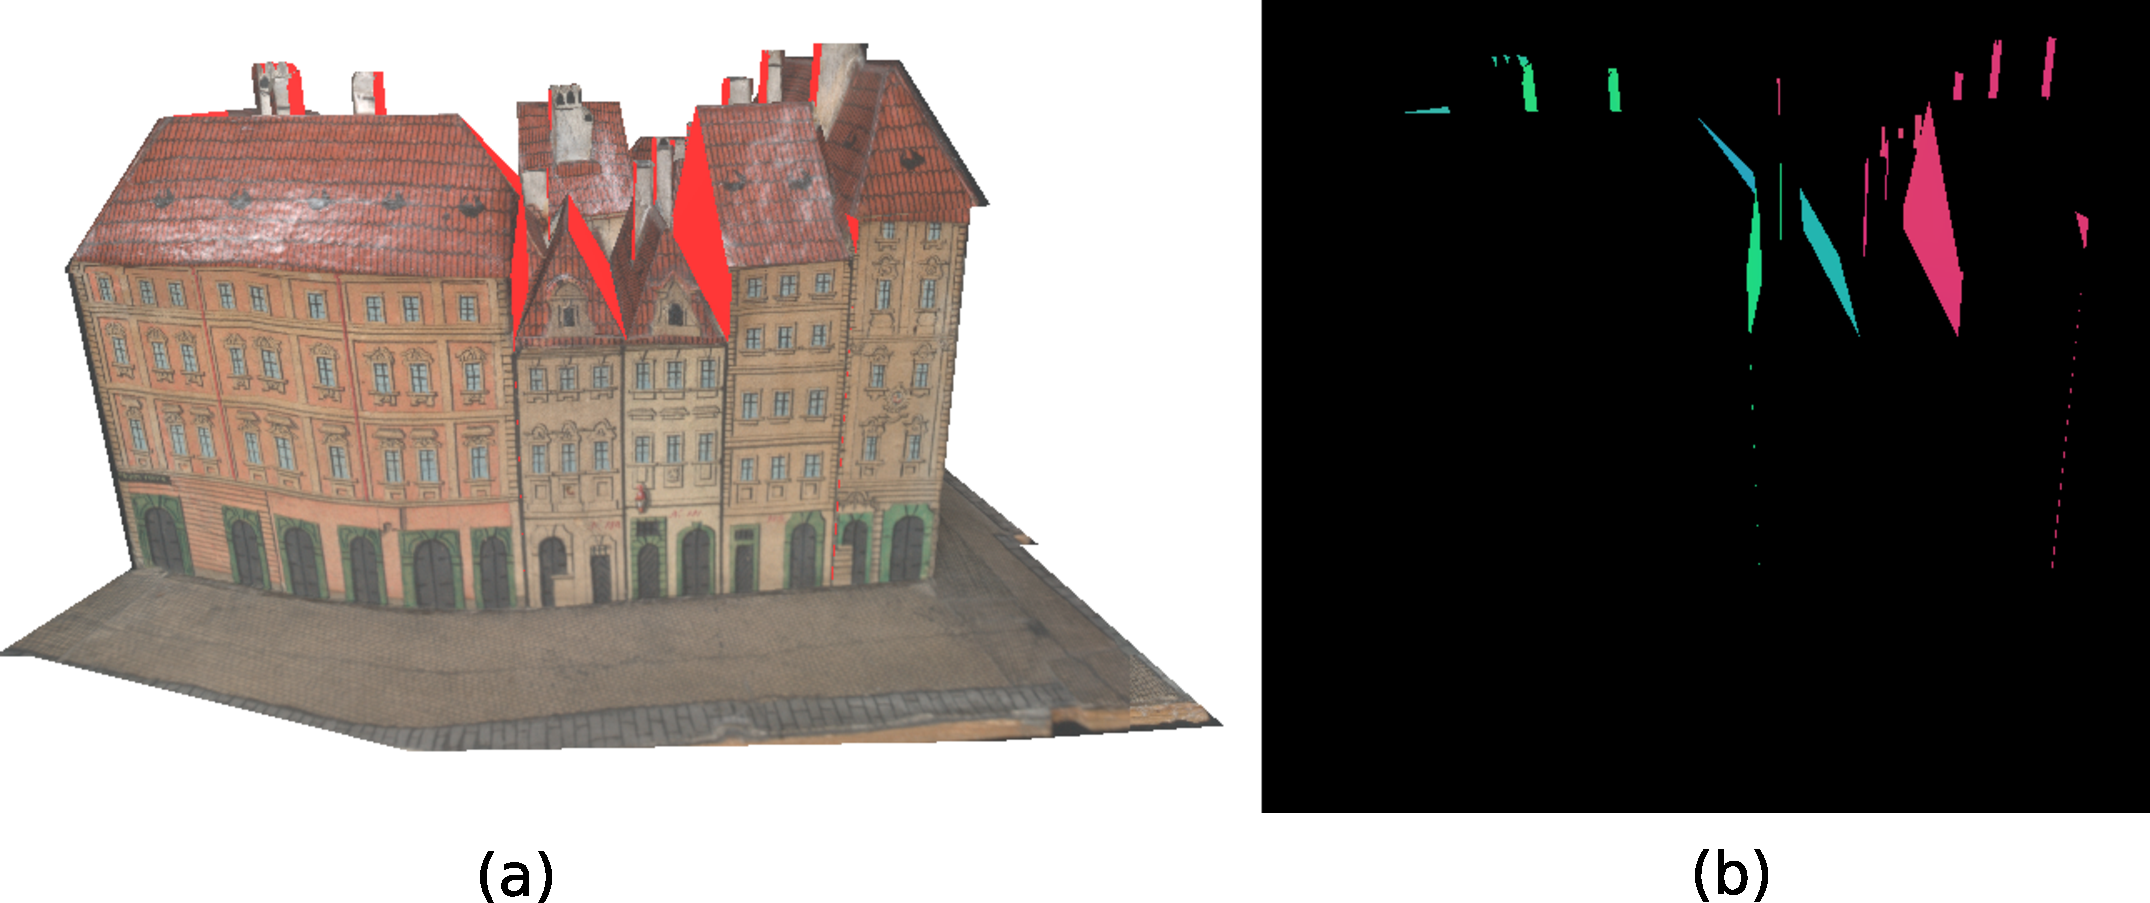
\includegraphics[width=\textwidth]{figures/faces-no-tex}
\caption{(a) Model otexturovaný šesti fotografiemi z kamer, které nejlépe odpovídají pohledu virtuální kamery. Červeně jsou zvýrazněny plochy, které nejde z kamer kvalitně otexturovat. (b) Vyrenderovaná textura s uloženými normálami v prvním průchodu algoritmu ze stejného pohleduj jaklo (a).}
\label{fig:faces-no-tex}
\end{center}
\end{figure}

K efektivnímu nalezení těchto ploch navrhujeme dvou průchodový algoritmus. Nejprve se vybere daný počet fotografií, které nejlépe odpovídají aktuálnímu pohledu. Poté se v prvním průchodu model vykreslí a zjistí se, které plochy je s daným prahem možné z vybraných fotografií otexturovat. Pokud fragment není možné pokrýt žádnou fotografií, vykreslí se do textury aktuální normála. V prvním průchodu tedy vznikne textura, která obsahuje normály ploch, které je nutné pokrýt, obr. \ref{fig:faces-no-tex} (b). Poté je provedeno klastrování těchto normál a jsou určeny nejvýznamnější směry. Tento přístup je vhodný, protože klastrování jde efektivně provést na GPU bez nutnosti přenosu velkého množství dat mezi GPU a CPU. Poté se vyberou nové fotografie, které nejlépe odpovídají nalezeným směrům (kamery, jejichž směr pohledu je opačný k nalezeným normálám). V druhém průchodu se poté provede výsledný rendering. 

\subsection{Texturování z více fotografií}
\label{sec:fragment-texturing}
Během renderingu je nutné vyřešit, jak budou otexturovány fragmenty, pro které je možné použít data z více fotografií. Princip je velmi podobný, jako při výběru fotografií, ale snahou při texturování je také omezení vzniku švů a omezení chybného otexturování zastíněných oblastí. Během texturování se již používají pouze fotografie, které byly vybrány v předchozím kroku.

Pro každou fotografii je vypočtena váha, fotografie s nejvyšší váhou je použita pro otexturování. Jeden fragment je otexturován pouze z jedné fotografie, není použito žádné vážené míchání barev z více fotografií. To vede k tomu, že dva sousední pixely mohou být vybrány z různých fotografií a tím mohou vznikat viditelné švy. Vážené míchání barev, jako např. v \cite{Debevec96} vede k rozmazání textur a na testovacích datech k vizuálně horšímu výsledku. 

Váha $w_i$ $i$-té fotografie je složena z několika faktorů. V úvahu je brána shoda směru kamery $d_c$ se směrem virtuální kamery $d_v$, stejně jako při výběru fotografií. Dále se uvažuje úhel mezi směrem kamery a normálou plochy $N_f$. Tím se preferují kamery s co nejvíce kolmým pohledem na danou plochu a zároveň je pravděpodobnější, že celá plocha bude otexturována z jedné fotografie. Nakonec je do výpočtu zahrnuta  velikost plochy $s_i$, kterou na fotografii zabírá model, viz výpočet konvexní obálky v sekci \ref{sec:photo-choosing}. Celkový výpočet váhy shrnuje následující rovnice:

\begin{align}
\label{eq:weight-scheme}
w_i &= dot(d_v, d_c) \times \left(\frac{1 + dot(-N_f, d_c)}{1 - cos(\alpha)} + 1\right) \times s_i \times \delta(i)\\
\delta(i) &= \left\{
  \begin{array}{l l}
    1 & \quad \text{pokud~$\exists P_i:(x, y, z) \to (s, t)$}\\
    0 & \quad \text{v opačném případě}
  \end{array} \right.
\end{align}

\noindent kde $dot$ značí skalární součin dvou vektorů a $\alpha$ je limitní úhel, který určuje, zda je plochu možné z dané kamery otexturovat.

Musíme brát v úvahu, že máme dvě rozdílné množiny fotografií. Nejprve jsme vybrali fotografie, které nejlépe odpovídají aktuálnímu pohledu. Poté jsme nalezli doplňující fotografie, které pokryjí zbývající plochy. Proto musí rendering probíhat ve dvou částech. Nejprve se aplikuje původní množina fotografií. Až poté se použijí doplňující fotografie, které mohou otexturovat pouze fragmenty, které se nepodařilo otexturovat v první části. Tímto se jednak preferují fotografie blízké aktuálnímu pohledu a zároveň se omezí situace, kdy by doplňující fotografie mohly chybně otexturovat plochy, které jsou z jejich pohledu zastíněné. K tomu i tak může dojít, ale pouze ve velmi omezených částech výsledného renderu, vizuálně to tedy nebude příliš výrazné. 


\chapter{Implementace}
\label{chap:impl}
\section{Požadavky na implementaci}

Aplikace by měla provádět texturování v reálném čase, proto je základním požadavkem rychlost zobrazování. Pro programy zobrazující 3D grafiku se jako dostatečná frekvence zobrazování snímků uvažuje 30fps. Dalším důležitým požadavkem je kvalita výsledných textur, která by měla být co nejlepší. To znamená zejména minimální výskyt švů mezi texturami a omezení chybného otexturování zastíněných oblastí. V optimálním případě by se render modelu z místa shodného s pozicí některé vstupní kamery neměl lišit od pořízené fotografie. Mezi další požadavky patří přenositelnost programu na více platforem a jednoduché ovládání pomocí grafického rozhraní.

\section{Použité technologie a knihovny}
Aplikace je implementována v ANSI C++11 a je možné ji přeložit v linuxových operačních systémech i v MS Windows. Základ aplikace je postaven na multiplatformní knihovně Qt 4.8. Qt je jedna z nejrozšířenějších knihoven pro tvorbu aplikací s grafickým rozhraním (GUI), ale poskytuje i další podpůrné moduly, které s grafickým rozhraním přímo nesouvisí. Kromě tvorby GUI je Qt využito pro načítání vstupů z periférií a pro správu vláken. Pro efektivní zobrazování 3D grafiky je využito OpenGL, které poskytuje API pro rendering a výpočty na grafickém procesoru (GPU). Společně s OpenGL je použit jazyk GLSL, který slouží k tvorbě tzv. shaderů. To jsou samostatné programy, které se spouští na grafické kartě a řídí jednotlivé části programovatelného zobrazovacího řetězce. Pro běh aplikace je nutná grafická karta podporující OpenGL 4.0, což je jakákoliv novější grafická karta. Část programu využívá OpenGL 4.3, ale pro základní funkčnost aplikace není tato verze vyžadována. 

Společně s OpenGL je využita knihovna GLEW 1.9, která slouží k načítání OpenGL rozšíření. S OpenGL je také úzce spjatá knihovna GLM, která poskytuje matematické operace běžně používané v počítačové grafice. Knihovna poskytuje základní datové struktury jako jsou vektory a matice a různé algebraické operace s těmito strukturami. Další použité knihovny jsou libjpeg 8 pro efektivní načítání obrázku ve formátu JPG a Assimp 3 pro načítání 3D modelů ve velkém množství formátů. Všechny využité knihovny jsou dostupné pod otevřenou licencí.

\section{Architektura aplikace}

Architektura aplikace zobrazující 3D grafiku v reálném čase se liší od běžných desktopových aplikací. Základem je efektivně využít zobrazovací řetězec a zajistit distribuci dat mezi aplikací a grafickou kartou tak, aby byly omezeny přenosy dat mezi CPU a GPU, které jsou velmi drahé. Zároveň je důležité, aby všechny zobrazovací průchody měly přístup k aktuálním datům potřebným pro rendering. Samotné OpenGL je možné popsat jako data-driven architekturu, nicméně aplikace využívá tradičního objektového návrhu. Základním prvkem OpenGL aplikace je hlavní smyčka, která neustále provádí aktualizaci scény bez ohledu na uživatelské vstupy. Ty se obvykle ukládají do fronty a jsou zpracovány vždy na začátku každé iterace smyčky. Zjednodušený návrh architektury aplikace je zobrazený na obrázku \ref{fig:architecture}.

\begin{figure}[ht]
\begin{center}
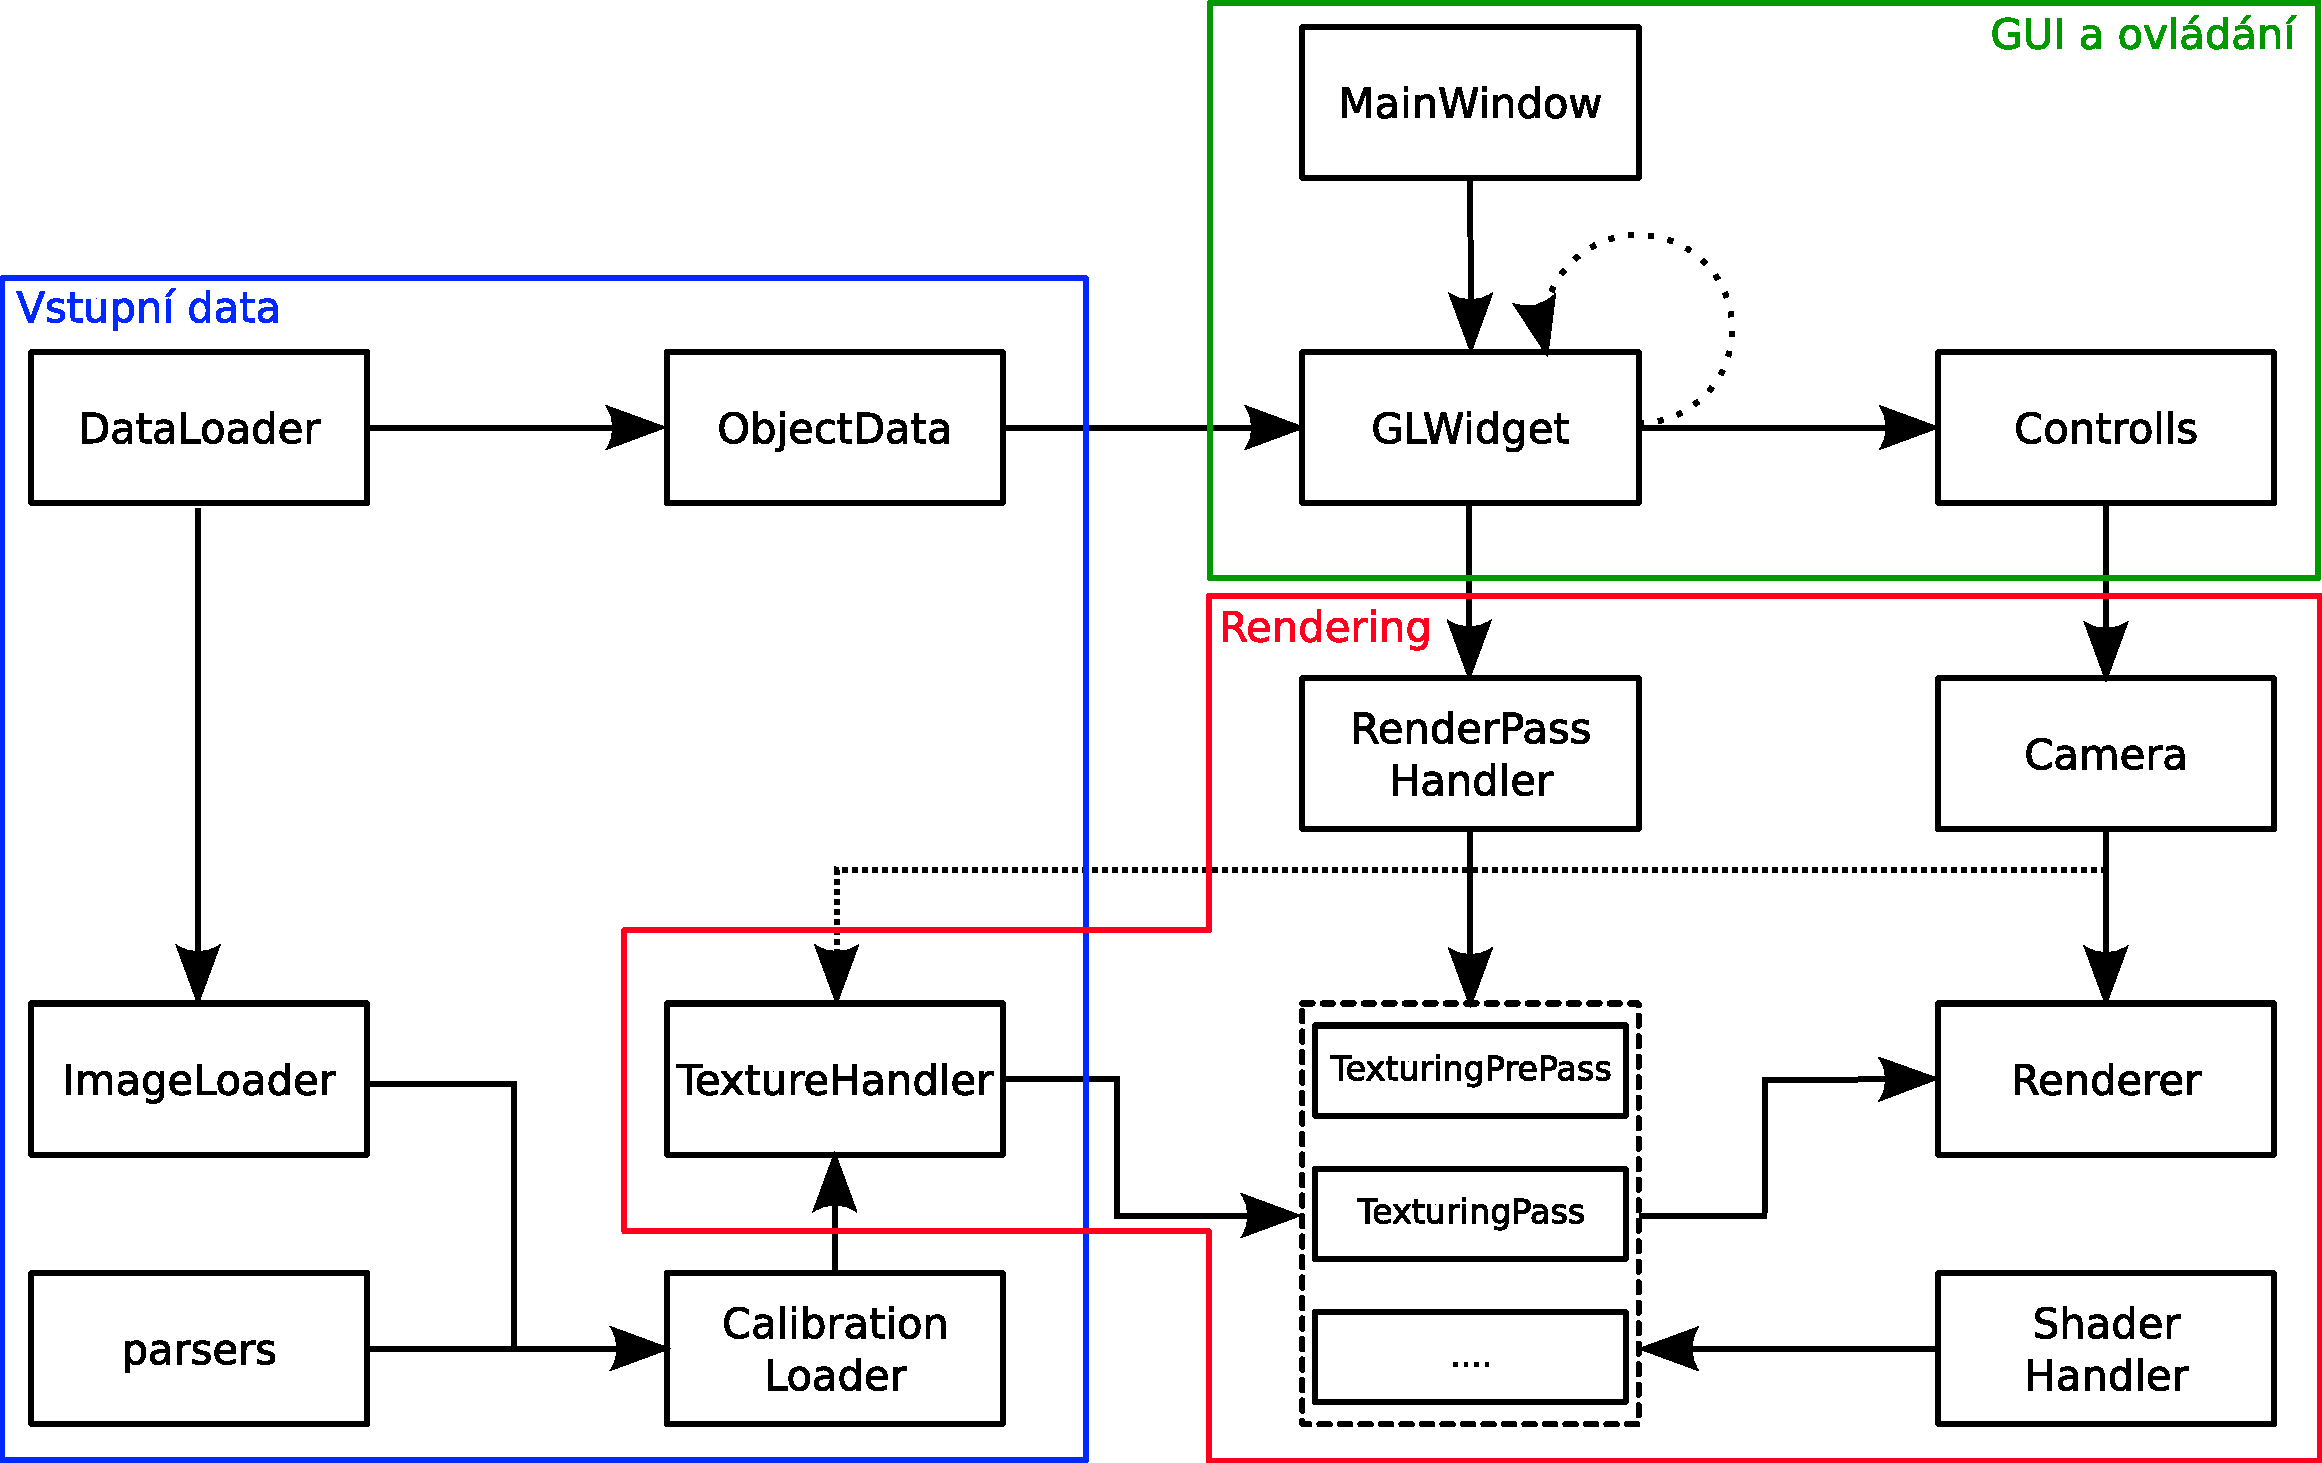
\includegraphics[width=\textwidth]{figures/architecture2}
\caption{Diagram ilustrující komunikaci základních komponent v aplikaci.}
\label{fig:architecture}
\end{center}
\end{figure}

Základem aplikace je třída \texttt{MainWindow}, která se stará o všechny komponenty GUI. Obsahuje aplikační menu a stará se o otevírání dialogových oken s nastavením programu. Jako centrální widget obsahuje třídu \texttt{GLWidget}, která má na starost zobrazování dat vykreslených pomocí OpenGL. Třída obsahuje metodu \texttt{paintGL}, která slouží jako hlavní smyčka, ve které se překresluje scéna. Zároveň se také třída  stará o vytvoření nové scény a inicializuje načtení vstupních dat. Design a používání GUI je detailněji popsáno v příloze \ref{chap:install}.


\section{Načítání a zpracování vstupních dat}

Aplikace na vstupu očekává 3D model a kalibrované fotografie. O načítání 3D modelu se stará třída \texttt{DataLoader} za pomoci knihovny Assimp. O načtení kalibrovaných fotografií se stará třída \texttt{CalibrationLoader}. Ta na základě zvoleného formátu vybírá parser pro načtení konfiguračních souborů s daty a stará se o přiřazení správných fotografií k načteným kamerám. Aplikace v současnosti podporuje dva formáty kalibrovaných dat:
\begin{itemize}
\item Bundler - výstupní soubor *.out z rekonstrukčního programu Bundler.
\item REALVIZ Ascii Camera - soubor *.rz3 s kalibračními daty a textový soubor, který k datům z rz3 souboru přiřazuje názvy fotografií.
\end{itemize}

Po načtení kalibrovaných fotografií dochází ke korekci pohledových směrů kamer. Vrcholy modelu jsou projekční maticí promítnuty do souřadnic ve fotografii. Z bodů, které leží uvnitř fotografie se vytvoří konvexní obálka pomocí Grahamova algoritmu \cite{Andrew79}.  Tento algoritmus má optimální asymptotickou složitost $O(n~log(n))$. Základem algoritmu je setřídění bodů podle souřadnice x, po setřídění je potřeba již pouze jeden průchod bodů se složitostí $O(n)$. Algoritmus začne s dvěma body s nejnižší x-ovou souřadnicí. Poté postupně prochází seřazené body a zjišťuje se, zda je vybraný bod nalevo nebo napravo od přímky, která prochází předchozí dvojicí vrcholů. Pokud je nalevo, druhý bod z dvojice nemůže ležet na konvexní obálce a je nahrazen nově nalezeným bodem. Tento proces pokračuje, dokud existuje bod nalevo od posledních dvou bodů na dočasné konvexní obálce. Algoritmus je možné snadno implementovat pomocí zásobníku. Body na dočasně nalezené konvexní obálce se vkládají na vrchol zásobníku. Pokud je nalezen bod vlevo od posledních dvou na zásobníku, odebírají se body ze zásobníku, dokud toto pravidlo opět neplatí. Poté se do zásobníku vloží nově nalezený bod a algoritmus pokračuje.

Po nalezení konvexní obálky je vypočítán centroid bodů na konvexní obálce. Pohledový vektor kamery je poté určen jako vektor procházející středem kamery a nalezeným centroidem. Zároveň je vypočtena plocha konvexní obálky pro pozdější použití při výpočtu váhy textury. Plochu lze snadno spočítat jako jednu polovinu determinantu matic, kde $n$ bodů na konvexní obálce je zapsáno do řádků matice a první bod se opakuje na konci, viz vztah \ref{eq:size}. Body musí být seřazené proti směru hodinových ručiček, což jde snadno zařídit již během Grahamova algoritmu. Po načtení kalibrací kamer následuje načtení samotných fotografií.

\begin{align}
\label{eq:size}
s_i = \frac{1}{2} 
\begin{vmatrix}
x_1 & y_1 \\
x_2 & y_2 \\
\vdots & \vdots \\
x_n & y_n \\
x_1 & y_1 \\
\end{vmatrix}
= \frac{1}{2} [(x_1 y_2 + x_2 y_3 + \ldots + x_n y_1) - (y_1 x_2 + y_2 x_3 + \ldots + y_n x_1)]
\end{align}

Vstupní fotografie jsou dodány v nejběžnějším formátu JPEG. Tento formát je však nevhodný pro textury, protože je komprimovaný, jeho načítání je netriviální a příliš pomalé. To by ani nebyl takový problém, pokud bychom fotografie načítali pouze jednou při spuštění aplikace. Problém je v tom, že fotografie mohou mít velké rozlišení a může jich být velké množství. Během testování byly použity scény s několika stovkami fotografií v rozlišení $4094\times4096$px. Takové množství fotografií v nekomprimovaném formátu zabere až desítky GB paměti. Nemůžeme proto očekávat, že je možné nahrát všechny fotografie do RAM a bude je nutné za běhu načítat z pevného disku. Z toho důvodu jsou při prvním načtení scény všechny fotografie načteny z původních JPG souborů a na disk se uloží každá fotografie také v nekomprimovaném formátu RAW. Při každém dalším spuštění se používají již nekomprimovaná data. Toto má nevýhodou v tom, že je nutné mít na disku dostatečné množství místa pro nekomprimovaná data. Nicméně pro běh aplikace v reálném čase je toto nezbytné.

Bohužel ani vytvoření RAW souborů není dostatečné pro načítání fotografií v reálném čase. Fotografie o v rozlišení 16MPx má v nekomprimovaném formátu velikost přibližně 45MB. Moderní HDD jsou schopné číst data rychlostí přibližně 150MB/s \cite{hdd}, to znamená, že načtení fotografie z HDD bude trvat minimálně 0.3 sec. I když budeme uvažovat moderní SSD disky s rychlostí čtení přes 500MB/s \cite{ssd}, bude trvat načtení fotografie do RAM téměř 90ms. To je samozřejmě naprosto nepoužitelné pro zobrazování v reálném čase, kdy při 30 fps je nutné vyrenderovat celý snímek za 33ms.

Jako řešení se nabízí možnost předem načítat omezené množství fotografií, které se vejde do RAM, aby fotografie byla vždy již načtená ve chvíli, kdy je jí třeba použít. Toto jsme implementovali za pomoci kd-stromu, kdy se načítaly fotografie nejbližší k aktuální pozici. Toto řešení se ukázalo velmi neefektivní, protože nebylo možné načítat dostatečné množství fotografií pro pokrytí všech možných směrů pohybu kamery. Ve výsledku byl procesor vytížený neustálým načítáním fotografií a aplikace byla nepoužitelná. Proto jsme zvolili jiný přístup. Pro každou fotografii jsou vytvořeny náhledy o velikosti šířce 512px. Tyto náhledy je již možné nahrát do RAM pro všechny vstupní fotografie. Při texturování se poté využívají náhledy a originální fotografie je načtena pouze v případě, kdy je opravdu použita. To vede ke snížení kvality textur při změně pohledu virtuální kamery, ale pokud se pohled virtuální kamery příliš nemění, textury v plném rozlišení se načtou poměrně rychle (konkrétní hodnoty jsou uvedeny v kapitole testování v sekci TODO).

O načítání fotografií se stará třída \texttt{TextureHandler}. Tato třída má primárně za úkol vybírat správné fotografie pro texturování. Při výběru jsou nejprve seřazeny fotografie podle shody s aktuálním pohledem a poté jsou vybrány fotografie s největší shodou. Shoda úhlů je počítána jednoduše pomocí skalárního součinu vektorů, který pro normalizované vektory vrací cosinus úhlu mezi vektory. Pokud je zapnutý průchod pro doplňování neotexturovaných ploch, polovina ze zadaného počtu fotografií pro texturování se vybere podle aktuálního směru a druhá polovina se rozdělí mezi neotexturované plochy. Pokud je potřeba dotexturovat plochy z více směrů, počet fotografií se rozdělí váženě podle velikostí daných ploch. Poté, co je fotografie určena k použití, se inicializuje načítání originální fotografie v plné velikosti. Toto je realizováno vícevláknově za použití třídy \texttt{QThreadPool} z Qt, která si interně udržuje frontu fotografií čekajících na načtení.  Při rychlém pohybu virtuální kamery se může stát, že fotografie již není aktuální dříve, než se uvolní volné vlákno a začne se načítat. Taková situace je ošetřena booleovskou hodnotou u každé fotografie, která indikuje zda se aktuálně fotografie používá. Pokud by nebylo toto ošetřeno, mohlo by dojít k načítání fotografií, které již nejsou vůbec potřeba, na úkor aktuálních. Zároveň je také nutné hlídat, které fotografie se přestaly používat. Tyto fotografie je nutné z paměti odstranit, jinak by postupně došlo k zaplnění paměti.

Třída se zároveň spravuje texturovací objekty, které slouží k připojení textur do OpenGL. Protože v OpenGL je omezené množství texturovacích jednotek, implementace má omezené maximální množství fotografií, které mohou být současně použity pro texturování. OpenGL garantuje minimálně 16 texturovacích jednotek\footnote{Ve skutečnosti OpenGL garantuje 16 texturovacíh jednotek pro každou fázi zobrazovacího řetězce, ale protože texturování provádíme pouze na fragmentovém shaderu, zajímá nás pouze množství texturovacích jednotek dostupné v této fázi.}, ale běžně GPU podporují 32 nebo více texturovacích jednotek, což je pro potřeby aplikace dostatečné. Problém ale nastává v tom, že do paměti na GPU není možné nahrát všechny náhledy. Pokaždé, když je fotografie vybrána, je nutné nahrát do GPU náhled a později i plnou velikost. Toto se samozřejmě neděje v každém framu, \texttt{TextureHandler} si udržuje přehled o tom, které fotografie jsou v GPU nahrány. Přenosy na GPU jsou prováděny pouze pokud byla vybrána nějaká nová fotografie. V takovém případě některá z textur na GPU přestala být aktuální.  \texttt{TextureHandler} se postará o to, aby se negenerovala nová textura, ale použije se existující texturovací objekt, pouze se přepíšou obrazová data. 

\newpage
\section{Rendering}

V aplikaci je implementováno několik renderovacích průchodů. O správu texturovacích průchodů se stará třída \texttt{RenderPassHandler}. Třída umožňuje přidávat a odebírat průchody a deleguje vykreslení objektu jednotlivým průchodům ve správném pořadí. Jednotlivé průchody dědí z třídy \texttt{RenderPass}, která obsahuje společné prvky průchodů. O renderování dat se stará třída \texttt{Renderer}, která zapouzdřuje přenos dat na GPU a poskytuje jednotlivým průchodům jednotné rozhraní. O správu shaderů se stará třída \texttt{ShaderHandler}. Třída se stará o načítání, kompilaci a linkování shaderů a ukládá si jejich identifikátory, které poté poskytuje renderovacím průchodům.

\subsection{Texturovací průchod}

Základním průchodem je \texttt{TextuingRenderPass}, který se stará o texturování modelu. Tento průchod zavolá aktualizaci třídy \texttt{TextureHandler}, od které obdrží aktuální fotografie společně s jejich kalibracemi. Protože vstupní fotografie mohou mít libovolné rozměry, jsou použity textury typu \verb|GL_TEXTURE_RECTANGLE|, které nemusí být čtvercové a jejich rozměry nemusí být zarovnané na mocniny 2. Jejich další výhodou je, že na shaderech se do těchto textur nepřistupuje pomocí normalizovaných souřadnic, ale přímo pomocí souřadnic v pixelech. To je výhodné, protože po promítnutí pozice fragmentu do obrázku pomocí matice kamery získáme souřadnice také v pixelech a nemusíme je normalizovat. Nevýhodou těchto textur je absence mipmap.

Kromě textur je do shaderu nutné připojit informace o kameře. To je realizováno pomocí uniformního bufferu. Tyto buffer slouží k rychlému nahrávání vetšího množství uniformních dat do shaderů. Uniformní buffer je umístěn v lokální paměti, proto je čtení dat z bufferu rychlé, což je na shaderu velmi důležité. Navíc je optimalizovaný pro sekvenční přístup, který je při iteraci kamer na shaderu vhodný. Buffer používá \texttt{std140} layout, který definuje přesné zarovnání datových typů, to umožňuje snadnou správu paměti v bufferu.


\lstset{
	morekeywords={TextureData,ivec2, vec3, vec2,in,out,mat4},
	emph={[1]projectCoords,inRange,computeWeight,dot,},
	emphstyle={[1]\color{red!30!black!}},
}
\begin{lstlisting}[caption={Výpočet váhy a projekce souřadnice na fragmentovém shaderu.},label={code:frag-weight},float=[ht]]
struct TextureData {
	mat4	u_Rt;						//matice R|t
	vec3	u_cameraViewDir;//opraveny smer kamery
	ivec2	u_textureSize;	//rozmery fotografie
	float	u_textureFL;		//ohniskova vzdalenost
	float	u_coveredArea;	//normalizovana plocha objektu ve fotce
};
layout(std140) uniform u_textureDataBlock {
	TextureData ub_texData[MAX_TEXTURES];
};

void projectCoords(in int index, in vec4 pos, out vec2 coords) {
	TextureData data = ub_texData[index];
	vec3 c = (data.u_Rt * pos).xyz;
	coords =  c.xy/c.z * data.u_textureFL + data.u_textureSize.xy * 0.5f;
}

bool inRange(in int index, in vec2 coords) {
	ivec2 s = ub_texData[index].u_textureSize;
	return coords.x >= 0 && coords.x < s.x && coords.y >= 0 && coords.y < s.y; 
}

float computeWeight(in int index, in vec3 N, out vec2 coords, in float dl = dirLimit) {
	TextureData data = ub_texData[index];
	float weight = data.u_coveredArea;
	weight *= dot(u_viewDir, data.u_cameraViewDir);

	projectCoords(index, In.v_position, coords);
	weight *= float(inRange(index, coords));

	float dirDiff = dot(N, data.u_cameraViewDir);
	weight *= -(dirDiff + 1.f) / (1.f - dl) + 1;
	return weight;
}
\end{lstlisting}

\subsection{Průchod pro pokrytí scény}

Pokrytí celé scény pomocí vyhledávání neotexturovaných ploch je řešené jako samostatný průchod \texttt{TexturingPrePass}, který je vždy spuštěn před texturovacím průchodem. Texturovací průchod ale není závislý na prvním průchodu. To má velkou výhodu v tom, že první průchod může být volitelný, a je možné ho za běhu aplikace zapínat a vypínat. K tomu jsou dva hlavní důvody - první průchod je výpočetně poměrně náročný a výrazně zpomaluje běh aplikace, což může být problém na méně výkoném hardwaru. Dále tento průchod vyžaduje OpenGL 4.3 s rozšířením \texttt{GL\textunderscore NV\textunderscore shader\textunderscore atomic\textunderscore float}, které je v současnosti dostupné pouze na kartách od výrobce NVIDIA. Aplikaci je tedy možné používat i bez tohoto průchodu, ale v některých scénách budou výsledky vizuálně horší.

Jak již bylo popsáno v sekci \ref{sec:photo-choosing}, texturovací průchod nejprve zjistí, které plochy není možné otexturovat. To zjistí výpočtem váhy, která probíhá stejně jako v texturovacím průchodu. Pokud je váha 0, fragment nelze otexturovat. V tom případě se do textury vykreslí aktuální normála. Vykreslování do textury je v OpenGL standardní operace a jde realizovat jednoduše. Poté je potřeba texturu přečíst a zjistit, které směry jsou v textuře uloženy. To ale není úplně jednoduché, protože textura je uložena v paměti na GPU. Kopírovat texturu v každém framu do RAM je velmi náročné a real-time aplikaci nepoužitelné. Proto jsem se rozhodl provést klastrování normál na GPU pomocí výpočetních shaderů.

Výpočetní shadery jsou poměrně nová technologie, dostupná od OpenGL 4.3. Tyto shadery narozdíl od ostatních nepatří do zobrazovacího řetězce a nepodílí se přímo na renderingu. Naopak tyto shadery umožňují provádět na GPU obecné výpočty, které s grafikou vůbec nemusí souviset. Architektura GPU je masivně paralelní, proto je na GPU vhodné provádět pouze výpočty, které jdou ve velkém měřítku paralelizovat. Výpočetní shadery jsou podobné technologiím CUDA nebo OpenCL, které také slouží k provádění obecných výpočtů na GPU. Výhoda výpočetních shaderů spočívá v tom, že je velmi snadné je zapojit do aplikace, které již OpenGL používá, protože mapování bufferů či textur probíhá úplně stejně, jako u běžných shaderů. Zároveň výpočetní shadery také používají jazyk GLSL, který poskytuje řadu užitečných funkcí. 

Pro klastrování normál je použit algoritmus k-means \cite{Lloyd82}. Tento algoritmus na začátku rozdělí data náhodně do $k$ skupin. Poté spočítá centroid každého klastru a porovná prvky se všemi centroidy. Pokud je prvek blíže k některému centroidu z jiného klastru, je do tohoto klastru přesunut. Takto algoritmus iterativně pokračuje, dokud existuje prvek, který se v dané iteraci přesunuje do jiného clusteru. Případně je možné algoritmus ukončit po daném počtu iterací. Algoritmus je primárně určen pro klastrování bodů v prostoru, ale je možné ho použít i pro klastrování vektorů, kdy vzdálenost směrů určuje úhel mezi vektory. Pro algoritmus je předem nutné zadat počet klastrů, ale některé klastry mohou zůstat na konci algoritmu prázdné. Během testování se ukázalo, že dostatečný počet klastrů pro normály je 4. V běžných scénách není pravděpodobné, že by nebyly otexturovány plochy z více jak čtyř význačných směrů.

Algoritmus je vhodný pro paralelní implementaci na GPU. Pro každý pixel vstupní normálové textury se spustí jedno vlákno, které porovná úhel se všemi klastry a určí, zda se normála přesune do jiného klastru. Poté je nutné v rámci všech klastrů spočítat jejich centroid, tedy sečíst všechny normály v klastru a výsledek vydělit počtem normál. Tento krok jde také paralelizovat pomocí jednoho ze základních paralelních algoritmů - redukce.

Paralelní redukce je algoritmus, který umožňuje paralelně sečíst sekvenci čísel. Funguje tak, že v každé iteraci jedno vlákno sečte dvě unikátní a čísla a uloží částečný výsledek. Tím vznikne z $n$ prvků původní množiny $\frac{n}{2}$ částečných výsledků. Takto se rekurzivně pokračuje, dokud algoritmus nenajde výsledek. Běh algoritmu je znázorněna na obrázku \ref{fig:reduction}.

\begin{figure}[h]
\begin{center}
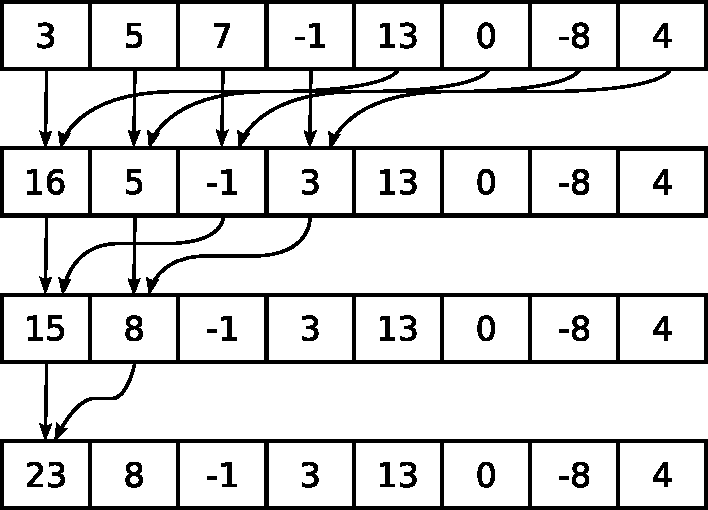
\includegraphics[width=\textwidth*2/3]{figures/reduction}
\caption{Obrázek znázorňuje paralelní redukci.}
\label{fig:reduction}
\end{center}
\end{figure}

Při spuštění výpočetního shaderu musíme explicitně zadat, kolik vláken chceme spustit. Vlákna se spouští v tzv. \emph{pracovních skupinách}, kdy vlákna v jedné pracovní skupině mohou vzájemně komunikovat pomocí sdílené paměti.  Pracovní skupiny jsou organizovány ve 3D mřížce, která usnadňuje indexování dat v mřížce. V rámci skupiny se nastavuje \emph{lokální velikost skupiny}, která určuje počet vláken spouštěných ve skupině. Tato lokální velikost je opět tří dimenzionální.  Pokud je tedy lokální velikost skupiny $(128, 1, 1)$, kterou spustíme v pracovní skupině velikosti $(4, 8, 16)$, spustíme 32768 vláken (instancí výpočetního shaderu). Každou instanci lze unikátně identifikovat pomocí systému vestavěných proměnných, které určují index vlákna v rámci lokální velikosti a index pracovní skupiny, ve které je vlákno spuštěno.

Pro zpracování normálové mapy je použita lokální velikost skupiny $(16, 16, 1)$ a počet pracovních skupin se dopočítává podle aktuálního rozlišení obrazovky. Textura je tedy zpracovávána po blocích $16\times16$ pixelů. Toho můžeme využít při inicializaci klastrů. Namísto toho, abychom v první iteraci normály náhodně rozdělili mezi klastry, můžeme vždy normály v jednom bloku vložit do jednoho zvoleného klastru. Protože se dá očekávat, že normály v jednom bloku budou velmi pravděpodobně patřit do jedné plochy, můžeme tímto klastrování urychlit. Po počátečním rozdělení je nutné spočítat centroidy klastrů, to provedeme pomocí výše popsané paralelní redukce. 

Paralelní redukce je provedena v rámci každé pracovní skupiny ve sdílené paměti. Sdílená paměť je velmi rychlá, proto je pro tento typ operace vhodná. Protože máme 4 clustery, nejde provést redukce jednoduše v rámci jednoho pole, protože v částečných součtech během redukce by nešlo určit, která data patří do jakého klastru. Proto je nutné vytvořit pro každý klastr jedno pole s počtem prvků stejným jako je lokální velikost skupiny. V ukázce \ref{code:comp-data} jsou deklarace polí, které se během redukce využívají. Deklarace označené klíčovým slovem \texttt{buffer} jsou v hlavní paměti GPU a jsou přístupné ze všech vláken. Pole označená jako \texttt{shared} jsou ve sdílené paměti, do které mají přístup pouze vlákna v rámci jedné pracovní skupiny.


\lstset{
	morekeywords={uint,coherent,restrict,buffer,layout,Cluster,shared},
}
\begin{lstlisting}[caption={Datové struktury potřebné pro sečtení normál pomocí paralelní redukce.},label={code:comp-data},firstnumber=1,float=[ht]]
struct Cluster {
	vec3 cntr;
	uint size;
};
coherent restrict layout(std430, binding = 0) buffer destBuffer {
	Cluster clusters[CLUSTERS];
	bool moving;
};
coherent restrict layout(std430, binding = 1) buffer idxBuffer {
	uint indices[];
};

shared vec3 cache[CLUSTERS][SIZE];
shared uint sizeCache[CLUSTERS][SIZE];
\end{lstlisting}


V ukázce \ref{code:comp-reduction} je zobrazen kompletní algoritmus paralelní redukce. Na řádcích \texttt{1-7} je provedena inicializace dat ve sdílené paměti. Všechna data jsou inicializována na 0, poté jsou inicializována data jednotlivých klastrů. Proměná \texttt{centroidIDX} je index klastru, do kterého přísluší aktuální vlákno. Tato proměnná je v prvním průchodu inicializovaná na základě pozice pracovní skupiny, v dalších iteracích je hodnota načtena z pole \texttt{indices}. Následuje cyklus, který provádí samotnou redukci odděleně pro každý klastr. Po každém cyklu je nutné provést paměťovou synchronizaci vláken pomocí funkce  \texttt{memoryBarrierShared}, která zajistí viditelnost zapsaných výsledků pro všechny vlákna. Zároveň je nutné provést synchronizaci pomocí \texttt{barrier}, která zajistí, že žádné vlákno v rámci skupiny nebude pokračovat, dokud všechny vlákna nedosáhly bariéry. Podmínku na řádce \texttt{21} vždy splní pouze jedno vlákno v pracovní skupině. Toto vlákno přidá pomocí atomické operace výsledek z redukce v dané skupině do bufferu v hlavní paměti. Tím získáme finální výsledek redukce. Atomické operace jsou velmi náročné a je vhodné se jim vyhýbat. V tomto případě je ale atomická operace nad proměnnou provedena pouze jednou pro každou pracovní skupinu, takže nezpůsobí výraznou ztrátu výkonu.

\lstset{
	emph={[1]barrier,memoryBarrierShared,atomicAdd},
}
\begin{lstlisting}[caption={Paralelní redukce na výpočetních shaderech.},firstnumber=1,label={code:comp-reduction},float=[ht]]
uint localID = gl_LocalInvocationIndex; //unikatni index v ramci skupiny
for(int i = 0; i < CLUSTERS; ++i) {
	sizeCache[i][localID] = 0;
	cache[i][localID] = vec3(0, 0, 0);
}
sizeCache[centroidIDX][localID] = int(isNormal);
cache[centroidIDX][localID] = int(isNormal) * N;

int stepv = (SIZE >> 1); 
while(stepv > 0) { //redukce v ramci skupiny
	if (localID < stepv) {
		for(int i = 0; i < CLUSTERS; ++i) {
			sizeCache[i][localID] += sizeCache[i][localID + stepv];
			cache[i][localID] += cache[i][localID + stepv];
		}
	}
	memoryBarrierShared(); //synchronizace vlaken
	barrier();
	stepv = (stepv >> 1);
}
if (localID == 0) { //secteni vysledku ze vsech skupin
	for(int i = 0; i < CLUSTERS; ++i) {
		if(sizeCache[i][0] != 0) atomicAdd(clusters[i].size, sizeCache[i][0]);
		if(cache[i][0].x != 0) atomicAdd(clusters[i].cntr.x, cache[i][0].x);
		if(cache[i][0].y != 0) atomicAdd(clusters[i].cntr.y, cache[i][0].y);
		if(cache[i][0].z != 0) atomicAdd(clusters[i].cntr.z, cache[i][0].z);
	}
}
\end{lstlisting}


Protože na výpočetních shaderech není možné synchronizovat všechna vlákna napříč pracovními skupinami, není možné po provedení redukce vydělit získaný centroid počtem vláken a pokračovat v klastrování. Jediný způsob, jak zajistit globální synchronizaci, je spustit nový shader. Proto jsou data z paralelní redukce zkopírována na CPU, kde proběhne výpočet a normalizace centroidu a poté je spuštěn nový shader, na kterém je provedeno klastrování. Přenos klastrů z GPU na CPU není problém, protože každý klastr obsahuje pouze jeden vektor a počet normál v klastru. Po výpočtu centroidu je spuštěn další shader, který provádí samotné klastrování. Shader má připojené stejné buffery, jako ten, který provádí redukci. Tento shader je již poměrně jednoduchý, pouze pro iteruje přes všechny klastry, porovnává úhel mezi aktuální normálou a centroidem klastru a nastavuje index nejvhodnějšího klastru, viz ukázka \ref{code:comp-cluster}. Poté se opět provede redukce a pokračuje se další iterací.

\lstset{
	emph={[1]memoryBarrier,dot},
}
\begin{lstlisting}[caption={K-means klastrování na výpočetních shaderech.},firstnumber=1,label={code:comp-cluster},float=[ht]]
float myDot = -1;

if(isNormal) {
	for(int k = 0; k < CLUSTERS; ++k) {
		memoryBarrier();
		float d = dot(N, clusters[k].cntr);
		if(d > myDot) {
			myDot = d;
			indices[id] = k;
			moving = true;
		}
	}
}
\end{lstlisting}

Klastrování je omezeno na 5 iterací. To se ukázalo jako dostatečné, protože klastry jsou v datech obvykle výrazné a algoritmus konverguje ke správnému rozdělení velmi rychle.

\subsection{Další průchody}

V aplikaci jsou implementovány ještě některé další jednoduché průchody. Pro vizualizaci vstupních kamer a lepší orientaci ve scéně slouží \texttt{RadarRenderPass}, který v rohu okna zobrazuje 2D pohled na scénu shora, kde jsou znázorněny pozice a směry všech vstupních kamer a také pozice virtuální kamery. Dále jsou zde zvýrazněné aktuálně využívané kamery pro texturování. \texttt{CameraPointsRenderPass} do scény umožňuje vykreslit body na pozice vstupních kamer, to je vhodné zejména pro kontrolu správného načtení vstupních dat a testování.

\chapter{Testování}
\label{chap:testing}


\chapter{Závěr}
\label{chap:end}


\renewcommand\refname{Zdroje}
\bibliographystyle{alpha}
\def\CS{$\cal C\kern-0.1667em\lower.5ex\hbox{$\cal S$}\kern-0.075em $}
\bibliography{zdroje}


\appendix


\chapter{Seznam použitých zkratek}

\begin{description}
\item[API]
\item[CPU] Central processing unit, procesor
\item[GPU] Graphic processing unit, grafický procesor
\item[HDD] Hard disk drive, pevný disk
\item[SSD] Solid-state drive
\item[GUI] Graphics user interface, grafické uživatelské rozhraní
\item[JPEG]  Joint photographic experts group
\item[fps]  frames per second, obrázků za vteřinu
\end{description}

\chapter{Instalační a uživatelská příručka}
\label{chap:install}

\section{Překlad aplikace}
\section{Používání aplikace}

\chapter{Obsah přiloženého CD}


\end{document}
